% Turkish Journal of Mathematics sinifi (math.cls); icerik degismeden bu sablona uyarlanmistir.
\documentclass[10pt]{math}

% --- Math ---
\usepackage{amsmath,amssymb,amsfonts,mathrsfs,mathtools}
\numberwithin{equation}{section}
\allowdisplaybreaks
\setlength{\jot}{4pt}

% --- Graphics + color ---
\usepackage{graphicx}
\graphicspath{{figures/}{thesis/figures/}}
\usepackage[dvipsnames]{xcolor}

% --- Tables ---
\usepackage{booktabs}
\usepackage{array}
\usepackage{tabularx}
\usepackage{float}
\usepackage{placeins}

% --- Lists, microtype, code, TikZ ---
\usepackage{enumitem}
\usepackage{microtype}
\usepackage{listings}
\usepackage{upquote}
\usepackage[most]{tcolorbox}
\tcbuselibrary{listings,breakable,skins}
\usepackage{tikz}
\usetikzlibrary{calc,positioning,arrows.meta,decorations.pathreplacing,
                decorations.markings,matrix,fit,backgrounds,shapes.misc}
\emergencystretch=3em

% --- Theorems via amsthm (sinifin \proof tanimini etkisizlestir) ---
\makeatletter
\let\proof\@undefined
\let\endproof\@undefined
\makeatother
\usepackage{amsthm}

% --- Turkish (shorthands=off: "=" aktiflesmesini engeller) ---
\usepackage[shorthands=off,turkish]{babel}

% --- Modern listing renk paleti ---
\definecolor{codebg}{HTML}{F8F9FB}
\definecolor{codeframe}{HTML}{D9DEE7}
\definecolor{codenumber}{HTML}{8A8F98}
\definecolor{codekeyword}{HTML}{7A3E9D}
\definecolor{codestring}{HTML}{22863A}
\definecolor{codecomment}{HTML}{6A737D}
\definecolor{codecaption}{HTML}{2F343B}

% --- Python kod blokları ---
\lstdefinestyle{modernpython}{
    language=Python,
    basicstyle=\ttfamily\footnotesize,
    keywordstyle=\bfseries\color{codekeyword},
    stringstyle=\color{codestring},
    commentstyle=\itshape\color{codecomment},
    numbers=left,
    numberstyle=\scriptsize\color{codenumber},
    stepnumber=1,
    numbersep=9pt,
    showstringspaces=false,
    breaklines=true,
    breakatwhitespace=true,
    breakindent=0pt,
    postbreak=\mbox{\textcolor{codeframe}{$\hookrightarrow$}\space},
    columns=fullflexible,
    keepspaces=true,
    tabsize=4,
    upquote=true,
    literate={-}{{\char`\-}}1
             {ç}{{\c{c}}}1 {Ç}{{\c{C}}}1
             {ğ}{{\u{g}}}1 {Ğ}{{\u{G}}}1
             {ı}{{\i}}1 {İ}{{\.{I}}}1
             {ö}{{\"o}}1 {Ö}{{\"O}}1
             {ş}{{\c{s}}}1 {Ş}{{\c{S}}}1
             {ü}{{\"u}}1 {Ü}{{\"U}}1,
}

% --- Kabuk (bash) komutları ---
\lstdefinestyle{modernbash}{
    language=bash,
    basicstyle=\ttfamily\footnotesize,
    keywordstyle=\bfseries\color{codekeyword},
    stringstyle=\color{codestring},
    commentstyle=\itshape\color{codecomment},
    numbers=none,
    showstringspaces=false,
    breaklines=true,
    breakatwhitespace=true,
    breakindent=0pt,
    postbreak=\mbox{\textcolor{codeframe}{$\hookrightarrow$}\space},
    columns=fullflexible,
    keepspaces=true,
    tabsize=4,
    upquote=true,
    literate={-}{{\char`\-}}1
             {ç}{{\c{c}}}1 {Ç}{{\c{C}}}1
             {ğ}{{\u{g}}}1 {Ğ}{{\u{G}}}1
             {ı}{{\i}}1 {İ}{{\.{I}}}1
             {ö}{{\"o}}1 {Ö}{{\"O}}1
             {ş}{{\c{s}}}1 {Ş}{{\c{S}}}1
             {ü}{{\"u}}1 {Ü}{{\"U}}1,
}

\lstset{style=modernpython}

\newtcblisting[use counter=lstlisting]{pythoncode}[2][]{%
    enhanced,
    breakable,
    listing only,
    listing style=modernpython,
    colback=codebg,
    colframe=codeframe,
    boxrule=0.45pt,
    arc=1.6mm,
    outer arc=1.6mm,
    left=6.2mm,
    right=2mm,
    top=1.2mm,
    bottom=1.2mm,
    boxsep=0pt,
    before skip=0.9em,
    after skip=0.9em,
    title={Kod~\thetcbcounter. #2},
    fonttitle=\bfseries\small,
    coltitle=codecaption,
    colbacktitle=codebg,
    colframe=codeframe,
    attach boxed title to top left={xshift=2mm,yshift=-1.2mm},
    boxed title style={
        enhanced,
        colback=codebg,
        colframe=codebg,
        boxrule=0pt,
        boxsep=0.5mm,
        left=0.5mm,
        right=0.5mm,
        top=0mm,
        bottom=0mm,
    },
    #1
}

\newtcblisting{bashcode}[1][]{%
    enhanced,
    breakable,
    listing only,
    listing style=modernbash,
    colback=codebg,
    colframe=codeframe,
    boxrule=0.45pt,
    arc=1.6mm,
    outer arc=1.6mm,
    left=2.4mm,
    right=2mm,
    top=1.2mm,
    bottom=1.2mm,
    boxsep=0pt,
    before skip=0.7em,
    after skip=0.7em,
    #1
}

% --- Accent renkleri (yalnizca TikZ diyagramlarinda kullanilir) ---
\definecolor{accent}{RGB}{59,91,146}
\definecolor{accentsoft}{RGB}{155,180,216}
\definecolor{oddsign}{RGB}{138,40,132}

% --- Hyperref (TJM sablonu: cite mavi, url siyah) ---
\usepackage[colorlinks=true,linkcolor=black,citecolor=blue,urlcolor=black]{hyperref}

% --- Theorems (amsthm, Turkce etiketler, sade journal stili) ---
\theoremstyle{plain}
\newtheorem{theorem}{Teorem}[section]
\newtheorem{proposition}[theorem]{Önerme}
\newtheorem{lemma}[theorem]{Lemma}
\newtheorem{corollary}[theorem]{Sonuç}
\theoremstyle{definition}
\newtheorem{definition}[theorem]{Tanım}
\newtheorem{example}[theorem]{Örnek}
\newtheorem{remark}[theorem]{Not}
\renewcommand{\proofname}{Kanıt}
\renewcommand{\lstlistingname}{Kod}
\makeatletter
\renewenvironment{abstract}{%
  \vskip .4em
  \small\noindent
  {\bf Öz:$\mbox{\!}$}%
}{}
\renewcommand{\keywords}[1]{\par\vskip 0.2cm \noindent{\bf Anahtar Kelimeler:} #1}
\AtBeginDocument{\renewcommand{\thelstlisting}{\arabic{lstlisting}}}
\makeatother

% --- Macros ---
\renewcommand{\sl}{\mathfrak{sl}}
\newcommand{\gfrak}{\mathfrak{g}}
\newcommand{\Uq}{U_q(\sl_2)}
\newcommand{\K}{\mathbb{K}}
\newcommand{\Q}{\mathbb{Q}}
\newcommand{\C}{\mathbb{C}}
\newcommand{\Z}{\mathbb{Z}}
\newcommand{\R}{\mathbb{R}}
\newcommand{\GL}{\mathrm{GL}}
\newcommand{\SL}{\mathrm{SL}}
\newcommand{\End}{\mathrm{End}}
\newcommand{\id}{\mathrm{id}}
\newcommand{\eps}{\varepsilon}
\newcommand{\cop}{\Delta}
\newcommand{\Dop}{\Delta^{\mathrm{op}}}
\newcommand{\qint}[1]{[#1]_q}
\newcommand{\qfact}[1]{[#1]_q!}
\newcommand{\qbin}[2]{\genfrac{[}{]}{0pt}{}{#1}{#2}_q}
\newcommand{\Vn}[1]{V_{#1}}
\newcommand{\hwt}{v_0}
\newcommand{\Rcheck}{\check{R}}

% --- TikZ ortak stilleri (diyagramlar) ---
\tikzset{
  strand/.style={line width=1pt, accent!80!black},
  rbox/.style={draw=accent!70!black, fill=accentsoft!55, rounded corners=2pt,
               line width=0.8pt, minimum height=6mm},
  rdot/.style={circle, fill=accent, inner sep=1.6pt},
  knode/.style={circle, draw=accent!70!black, fill=accentsoft!45,
                line width=0.8pt, minimum size=7mm, font=\small},
  kedge/.style={accent!70!black, line width=0.9pt},
  faredge/.style={oddsign!75!black, line width=0.9pt, densely dashed},
  glabel/.style={font=\footnotesize, accent!60!black},
}

% --- TJM ust-verisi ---
\yil{2026}
\vol{}
\fpage{}
\lpage{}
\doi{}

\title{Quantum Grup Yapılarının Python Ortamında Modellenmesi}

\newcommand{\orcidicon}[1]{\href{#1}{\protect\raisebox{-0.15ex}{
\includegraphics[height=1.7ex]{orcid.png}}}}
\author[ÇELİK and TEREKLİ]{%
\textbf{Prof. Dr. Salih ÇELİK$^{1}$\,\orcidicon{https://orcid.org/0000-0002-6590-1032},
Taha Berk TEREKLİ$^{1}$\,\orcidicon{https://orcid.org/0009-0004-8266-1116}}\\[0.35em]
$^{1}$Matematik Bölümü, Yıldız Teknik Üniversitesi, İstanbul, Türkiye%
}

% Ilk sayfa altbilgisi: dergi logosu/lisans notu yok, yalnizca sayfa numarasi
\makeatletter
\def\ps@myheadings{%
  \def\@oddhead{}%
  \let\@evenhead\@oddhead
  \def\@oddfoot{\normalfont\hbox to \textwidth{\hfil \thepage}}%
  \def\@evenfoot{\normalfont\hbox to \textwidth{\thepage \hfil}}%
  \let\@mkboth\@gobbletwo \let\sectionmark\@gobble \let\subsectionmark\@gobble
}
\makeatother

\begin{document}
\maketitle
\pagestyle{myheadings}

\begin{abstract}
Bu makale, Drinfeld--Jimbo kuantum grubu $\Uq$ ve $GL_q(2|1)$ kuantum
süpergrubu için temel temsil-teorik ve Yang--Baxter tipi bağıntıları
Python/SymPy ortamında yeniden üretilebilir biçimde modellemektedir. Yöntemin
çekirdeği, her cebirsel eşitliği açık sonlu boyutlu temsiller üzerinde bir
kalıntı matrisine indirgemek ve bu matrisin tüm girdilerini sembolik olarak
sadeleştirerek sıfır olup olmadığını denetlemektir.

$\Uq$ için sonlu boyutlu en yüksek ağırlıklı $V_n$ temsilleri açık matrislerle
kurulmuş; tanımlayıcı bağıntılar, Hopf yapısı, tensör çarpımı eylemi ve
Clebsch--Gordan en yüksek ağırlık vektörleri seçilen temsiller üzerinde
sembolik olarak doğrulanmıştır. $V_1\otimes V_1$ üzerinde $R$-matrisi,
kuantum Yang--Baxter denklemi, örgü bağıntısı ve Hecke skein özdeşliği
sıfır-kalıntı yöntemiyle kontrol edilmiştir. $GL_q(2|1)$ tarafında ise
literatürde verilen $9\times 9$ $R$-matrisi bağımsız olarak kodlanmış,
$p(e_1)=p(e_2)=0$, $p(e_3)=1$ parite konvansiyonu ile süper permütasyon
kullanılarak $R_{13}$ yerleşimi kurulmuş ve graded Yang--Baxter kalıntısının
tüm $27\times 27$ girdilerinin sıfır olduğu matris girdileri düzeyinde
sembolik olarak doğrulanmıştır. Sonuçların her biri \texttt{pytest} tabanlı
testlere bağlanmıştır. Çalışmanın temel katkısı yeni bir kuantum grup tanımı
vermek değil, bilinen kuantum grup ve kuantum süpergrup yapılarını modüler,
test edilebilir ve yeniden üretilebilir bir sembolik doğrulama altyapısına
dönüştürmektir.

\keywords{kuantum gruplar, $U_q(\mathfrak{sl}_2)$, kuantum süpergruplar, $GL_q(2|1)$, Yang--Baxter denklemi, sembolik hesaplama}
\end{abstract}

\section{Giriş ve Motivasyon}

Kuantum gruplar, 1980'lerin ortasında V.~Drinfeld ve M.~Jimbo'nun --- istatistik
mekaniğin integrallenebilir modellerini ve bunların temelinde yatan
\emph{kuantum Yang--Baxter denklemini} cebirsel bir dile oturtma çabası içinde ---
birbirinden bağımsız olarak geliştirdiği Hopf cebirsel yapılardır
\cite{Drinfeld,Jimbo,Kassel,ChariPressley}. Adlarındaki ``grup'' sözcüğü
yanıltıcıdır: burada incelenen nesneler Lie grubu değil, evrensel sarmalayıcı
cebir $U(\gfrak)$'nin bir $q$ parametresi boyunca tek-parametreli
deformasyonlarıdır. Bu deformasyonlar genellikle ne değişmeli ne de
eş-değişmelidir; tam da bu nedenle temsillerin tensör çarpımında sıradan takasın
yerini örgülü bir yapı alır. Bu örgülü yapının cebirsel çekirdeğinde,
integrallenebilir sistemlerle düğüm değişmezlerini aynı matematiksel hat
üzerinde buluşturan Yang--Baxter denklemi ve onun çözümü olan $R$-matrisleri
bulunur \cite{Jones,Kassel}.

Bu denklemlerin somut temsiller üzerinde sağlandığını göstermek, $q$'ya bağlı
yüksek boyutlu matris çarpımlarını gerektirir; el ile yürütüldüğünde işlem hem
uzar hem de hataya açık hâle gelir. Burada izlenen yol, söz konusu cebirsel
manipülasyonları sembolik bilgisayar cebiriyle (Python/SymPy) modellemek, her
bağıntıyı bir sıfır-kalıntı matris testine indirgemek ve elde edilen sonuçları
otomatik birim testlere bağlamaktır. Anlatı iki eksende ilerler: \textbf{(i)}
$\Uq$ için temsil teorisi ve $R$-matrisi altyapısı; \textbf{(ii)} $GL_q(2|1)$
kuantum süpergrubu için graded Yang--Baxter doğrulaması.

Bu iki eksen, kuantum grupların temel prototipi $\Uq$ ile Salih Çelik ve
Sultan A.\ Çelik'in tanıttığı $GL_q(2|1)$ kuantum süpergrubunu beş doğrulama
başlığı altında ele alan ortak bir hedefte buluşur:
\begin{enumerate}[leftmargin=*]
  \item \textbf{Cebirsel}: dört tanımlayıcı bağıntının ve dokuz Hopf
        aksiyomunun (eş-birleşmelilik, eş-birim, antipot) matris düzeyinde
        sembolik doğrulanması.
  \item \textbf{Temsil teorik}: $(n+1)$-boyutlu indirgenemez temsil $V_n$'in
        açık inşası, $V_m \otimes V_n$ Clebsch--Gordan ayrışımının $q$-deforme
        katsayılarıyla hesaplanması.
  \item \textbf{Topolojik}: $V_1\otimes V_1$ üzerinde $R$-matrisinin
        inşası, kuantum Yang--Baxter denkleminin ve örgü bağıntısının
        sembolik matris doğrulaması; bu doğrulamanın düğüm değişmezleri (Jones
        polinomu) ile bağlantısı.
  \item \textbf{Asimptotik}: $q$ parametresinin üç farklı limitinde aynı
        temsilin yapısının nasıl değiştiğinin somut karşılaştırılması.
  \item \textbf{Süpergrup ve graded YBE}: Salih Çelik ve Sultan A.\ Çelik tarafından tanımlanan
        $GL_q(2|1)$ kuantum süpergrubunun $9\times 9$ $R$-matrisi kodlanarak,
        graded Yang--Baxter denklemi $27\times 27$ matris düzeyinde sembolik
        olarak doğrulanır.
\end{enumerate}

Bu çalışmanın özgün katkısı, yeni bir kuantum grup tanımlamak ya da
literatürdeki sınıflandırma sonuçlarını yeniden ispatlamak değildir. Katkı,
literatürde bilinen $\Uq$ ve $GL_q(2|1)$ yapılarını sonlu boyutlu temsiller
üzerinde yeniden üretilebilir, test edilebilir ve sembolik bir doğrulama
altyapısına dönüştürmektir. Bu kapsamda $\Uq$ temsilleri, tanımlayıcı
bağıntılar, Hopf aksiyomları, tensör çarpımları, Clebsch--Gordan en yüksek
ağırlık vektörleri, $R$-matrisi kontrolleri ve limit karşılaştırmaları aynı
paket içinde ele alınır. Ayrıca Salih Çelik ve Sultan A.\ Çelik'in
$GL_q(2|1)$ için verdiği $R$-matrisi bağımsız olarak kodlanır ve graded
Yang--Baxter denklemi, parite uyumlu $R_{13}$ yerleşimiyle $27\times 27$
matris girdileri düzeyinde doğrulanır. Raporlanan her sembolik eşitlik,
\texttt{pytest} tabanlı yeniden çalıştırılabilir bir teste bağlanır
\cite{SymPy,pytest}.

\paragraph{Yazar tercihleri ve yöntemsel konum.} $\Uq$ prototip olarak
seçilmiştir; çünkü sonlu boyutlu temsilleri açık matrislerle yazılabilir ve
klasik limit, tensör çarpımı, $R$-matrisi ve kristal gölge aynı örnek üzerinde
izlenebilir. $GL_q(2|1)$ ise graded durumda parite işaretlerinin hesaba nasıl
girdiğini gösteren yeterince küçük ama elle takip için yeterince hassas bir
örnektir. Kalıntı matrisleri, soyut eşitlikleri doğrudan test edilebilir
nesnelere çevirdiği için kullanılmıştır; \texttt{pytest} ise aynı hesabın depo
klonlandığında aynı komutla yeniden çalıştırılabilmesini sağlar. Elle en çok
hata üreten adımlar, özellikle $R_{13}$ yerleşimi, süper permütasyon işaretleri
ve yüksek tensör kuvvetlerinde faktör sıralamasıdır.

Çalışmanın yazılım ayağı, temel sembolik hesaplarda SymPy'yi kullanan modüler
\texttt{quantum\_group} paketidir; her doğrulama \texttt{pytest} testleriyle
otomatik biçimde yeniden çalıştırılabilir. Bu nedenle raporlanan eşitlikler,
ilgili testleri koşturan okuyucu tarafından aynı sonlu boyutlu matris modeli
üzerinde yeniden üretilebilir.

\paragraph{Makalenin akışı.} İlkin gerekli teorik zemin --- gruplar, Lie
cebirleri, Hopf cebirleri, $\Uq$ ve temsiller --- yoğun ama eksiksiz biçimde
verilir. Ardından yazılım mimarisi tanıtılır. Sonraki bölümler hesaplamalı
katkıları sırayla sunar: Clebsch--Gordan ayrışımı, $\Uq$ için $R$-matrisi ve
YBE, $GL_q(2|1)$ için graded Yang--Baxter doğrulaması ve üç asimptotik limit.
Kapanış bölümü bulguları toparlayıp ileri çalışma yönlerini sıralar.

\section{Teorik Arka Plan}

Bu bölüm, ileride kodla doğrulanacak eşitliklerin hangi standart cebirsel
zemine dayandığını sabitlemek için yazılmıştır. Gruplar, Lie cebirleri,
evrensel sarmalayıcı cebir ve Hopf yapısı burada yeni sonuç olarak değil,
$\sl_2 \to \Uq \to V_n$ hattında kullanılacak ortak dil olarak özetlenir.
Kuantum grup literatüründeki ayrıntılı arka plan için Kassel, Chari--Pressley
ve Lusztig'e başvurulabilir \cite{Kassel,ChariPressley,Lusztig}.

\subsection{Gruplar, Lie Cebirleri ve Evrensel Sarmalayıcı Cebir}

\begin{definition}
Bir \emph{grup} $G$, birleşmeli bir ikili işlem $\cdot : G \times G \to G$,
iki yanlı bir birim eleman $e \in G$ ve her elemanın bir tersi olan bir
küme yapısıdır.
\end{definition}

Sürekli simetri grupları üzerinde diferansiyel hesap yapabilmek için Lie
gruplarına geçilir: $G$ aynı zamanda düzgün bir manifolddur ve grup
işlemleri düzgündür. Klasik örnekler $\GL_n(\C)$, $\SL_n(\C)$,
$\mathrm{SO}_n$, $\mathrm{SU}_n$'dur. Bir Lie grubunun \emph{infinitezimal}
yapısı tanjant uzayında saklıdır.

\begin{definition}
Bir cisim $\K$ üzerinde bir \emph{Lie cebri} $\gfrak$, antisimetrik ve Jacobi
özdeşliğini sağlayan iki-doğrusal $[\,\cdot\,,\,\cdot\,] : \gfrak \times \gfrak \to \gfrak$
parantezi ile donatılmış vektör uzayıdır:
\[
  [x,y] = -[y,x], \qquad
  [x,[y,z]] + [y,[z,x]] + [z,[x,y]] = 0.
\]
\end{definition}

Matris Lie grupları için Lie parantezi komütatördür: $[x,y] = xy - yx$.
Lie grup ile Lie cebir arasındaki köprü üstel dönüşüm $\exp : \gfrak \to G$ ile
verilir. Lie cebrinin temsil teorisini lineerleştiren araç, bir sonraki
adımdır.

\begin{definition}
$\gfrak$ bir Lie cebri olsun. \emph{Evrensel sarmalayıcı cebir} $U(\gfrak)$,
$\gfrak$'yi içeren ve $xy - yx = [x,y]$ bağıntısı dışında hiçbir bağıntıya
tabi olmayan birleşmeli birimli cebirdir.
\end{definition}

$\gfrak$'nin temsilleri ile $U(\gfrak)$'nin temsilleri kanonik olarak birebir
karşılık gelir; ve kuantum gruba deformasyon hedefimiz tam olarak $U(\gfrak)$
nesnesidir, $\gfrak$'nin kendisi değil.

\subsection{$\sl_2$ Lie Cebri}

İz sıfır $2 \times 2$ kompleks matrisleri vektör uzayı $\sl_2(\C)$ üç
boyutludur ve standart bazı:
\[
  e = \begin{pmatrix} 0 & 1 \\ 0 & 0 \end{pmatrix},\qquad
  f = \begin{pmatrix} 0 & 0 \\ 1 & 0 \end{pmatrix},\qquad
  h = \begin{pmatrix} 1 & 0 \\ 0 & -1 \end{pmatrix}.
\]
Bu eleman üçlüsü temel bağıntıları sağlar:
\begin{equation}\label{eq:sl2-rels}
  [h,e] = 2e, \qquad [h,f] = -2f, \qquad [e,f] = h.
\end{equation}
Küçük boyutuna karşın $\sl_2$, yarı-basit Lie cebirlerinin yerel yapı
taşlarından biridir: basit kökler boyunca ortaya çıkan $\sl_2$ alt yapıları,
temsil teorisindeki birçok hesabı bu üç üreteçli modele indirger.

\begin{theorem}[$\sl_2$'nin sonlu boyutlu temsilleri]
$\sl_2(\C)$'nin sonlu boyutlu indirgenemez temsilleri, negatif olmayan
tamsayı $n \in \Z_{\geq 0}$ ile birebir karşılık gelir. $V_n$ adlı temsil
$(n+1)$-boyutludur, baz $\{v_0, v_1, \dots, v_n\}$ üzerinde
\[
  h \cdot v_k = (n - 2k) v_k, \quad
  f \cdot v_k = v_{k+1}, \quad
  e \cdot v_k = k(n-k+1)\, v_{k-1},
\]
ve sınır koşulları $f \cdot v_n = 0$, $e \cdot v_0 = 0$.
\end{theorem}

Bu standart sınıflandırma, kuantum gruba geçerken kullanılacak $V_n$ notasyonunu
sabitler. $h$'nin özdeğerleri olan $n - 2k$ tamsayılarına \emph{ağırlıklar}
denir; aynı veri kuantum modelde $K$-özdeğerleri olarak yeniden ortaya çıkacaktır
\cite{ChariPressley}.

\subsection{Hopf Cebirleri}

Bir cebir verildiğinde, onun temsilleriyle ne yapabileceğimiz tek başına çarpım
yapısıyla belirlenmez. İki temsilin tensör çarpımının yine bir temsil olması,
trivial (skaler) bir temsilin tanımlanabilmesi ve her temsile bir dual
eşlik edebilmesi --- bunların hiçbiri birleşmeli çarpımdan kendiliğinden çıkmaz.
Eksik olan, cebire eklenen üç ek dönüşümdür: bir elemanı iki kopyaya ``dağıtan''
eş-çarpım, skalere indirgeyen eş-birim ve tersleme rolünü üstlenen antipot. Bu
üçlü \emph{Hopf cebir} aksiyomlarını oluşturur ve aslında temsil teorisinin
tensör/dual işlemlerini cebirin içine gömme aracıdır \cite{Kassel}.

\begin{definition}
$\K$ cismi üzerinde birleşmeli birimli bir cebir $H$, eğer eş-çarpım
$\cop : H \to H \otimes H$, eş-birim $\eps : H \to \K$ ve antipot
$S : H \to H$ dönüşümleriyle donatılmış ve aşağıdakileri sağlıyorsa
\emph{Hopf cebri}'dir:
\begin{enumerate}[leftmargin=*]
  \item $(\cop \otimes \id) \circ \cop = (\id \otimes \cop) \circ \cop$ \quad (eş-birleşmelilik)
  \item $(\eps \otimes \id) \circ \cop = \id = (\id \otimes \eps) \circ \cop$ \quad (eş-birim)
  \item $\mu \circ (S \otimes \id) \circ \cop = \eps(\,\cdot\,)\,1 = \mu \circ (\id \otimes S) \circ \cop$ \quad (antipot)
\end{enumerate}
Burada $\mu$ cebir çarpımıdır; ayrıca $\cop$ ve $\eps$ cebir homomorfizmleri,
$S$ cebir anti-homomorfizmi olmak zorundadır.
\end{definition}

Hopf yapısının temsil teorik anlamı kritiktir:
\begin{itemize}[leftmargin=*]
  \item İki temsil $V$, $W$ verildiğinde, $V \otimes W$ üzerinde $H$-etkisi
        eş-çarpım aracılığıyla tanımlanır: $X \cdot (v \otimes w) := \cop(X) \cdot (v \otimes w)$.
  \item Eş-birim $\eps$, trivial temsil $\K$'ya karşılık gelir.
  \item Antipot $S$, dual temsil $V^*$'ı tanımlamak için kullanılır.
\end{itemize}

\begin{example}
Her $U(\gfrak)$, eş-değişmeli (cocommutative) bir Hopf cebridir; üreteçler
$x \in \gfrak$ üzerinde
\[
  \cop(x) = x \otimes 1 + 1 \otimes x, \quad \eps(x) = 0, \quad S(x) = -x.
\]
Eş-değişme, klasik tensör çarpımının değişmeli olmasının cebirsel
karşılığıdır. Kuantum grupta tam olarak bu özellik bozulacaktır.
\end{example}

\section{Kuantum Grup $\Uq$'nin Tanımı}

Drinfeld--Jimbo fikrinin özü, $U(\sl_2)$'nin Serre tipi bağıntılarını ayakta
tutarken Cartan üretecini bir grup-benzeri öğeye dönüştürmektir
\cite{Drinfeld,Jimbo}. Klasik
$h$ yerine tersinir bir $K = q^h$ değişkeni konur; bu sayede Cartan eylemi
``$q$ üssü'' biçiminde köşegenleşir ve $[e,f]=h$ bağıntısı, $\qint{h}$
ifadesiyle yumuşatılmış bir versiyona geçer. Deformasyon parametresi $q$, ayrı
bir cebirsel nicelik eklemez; var olan tüm yapı sabitlerini $q$'nun rasyonel
fonksiyonlarına taşır ve $q\to 1$ limitinde her şeyi klasik $U(\sl_2)$'ye geri
indirir.

Bu çalışmada $q$ çoğunlukla formel bir parametre olarak ele alınır ve sembolik
hesaplamalar $\Q(q)$ üzerinde yürütülür. Bir karmaşık değere özelleştirme
yapıldığında $q\in\C^\times$ ve tanımda görünen paydalar için $q\neq \pm 1$
varsayılır; birim köklerde ise temsil teorisinin değiştiği ayrıca
Bölüm~\ref{sec:limits} içinde belirtilir.

\begin{definition}\label{def:Uq}
$\Uq$ kuantum grubu, $\Q(q)$ üzerinde dört üreteç $E$, $F$, $K$, $K^{-1}$
ile aşağıdaki bağıntılara tabi birleşmeli cebirdir:
\begin{align}
  K K^{-1} &= K^{-1} K = 1, \tag{R1} \\
  K E K^{-1} &= q^{2} E, \tag{R2} \\
  K F K^{-1} &= q^{-2} F, \tag{R3} \\
  [E, F] := EF - FE &= \frac{K - K^{-1}}{q - q^{-1}}. \tag{R4}
\end{align}
\end{definition}

Bu cebir bir Hopf cebridir; üreteçler üzerinde:
\begin{align}
  \cop(E) &= E \otimes 1 + K \otimes E, \\
  \cop(F) &= F \otimes K^{-1} + 1 \otimes F, \\
  \cop(K) &= K \otimes K, \\
  \eps(E) &= \eps(F) = 0, \quad \eps(K) = 1, \\
  S(E) &= -K^{-1} E, \quad S(F) = -F K, \quad S(K) = K^{-1}.
\end{align}
Burada $\cop$ eş-\emph{değişmeli değildir}: $\tau \circ \cop \neq \cop$ (bunu
örgülü R-matrisin varlığı tam olarak kuantize edecek).

\subsection{$q$-Deformasyon Sezgisi}

$q$-tamsayılar şu formülle tanımlanır:
\begin{equation}\label{eq:qint}
  \qint{n} := \frac{q^n - q^{-n}}{q - q^{-1}} = q^{n-1} + q^{n-3} + \dots + q^{-(n-1)}.
\end{equation}
L'H{\^o}pital kuralıyla bakıldığında $q\to 1$ için $\qint{n}\to n$ olur; benzer
biçimde $q$-faktöriyel $\qfact{n} = \qint{n}\qint{n-1}\cdots\qint{1}$ klasik
$n!$'e yaklaşır. Burada kritik olan nokta şudur: $\qint{n}$ yalnızca süslü bir
sayı değil, deformasyonun \emph{işleyiş mekanizmasıdır}. Birazdan görüleceği
gibi, $V_n$ temsilinde $E$'nin matris katsayıları doğrudan
$\qint{k}\qint{n-k+1}$ çarpımlarıyla verilir; dolayısıyla klasik tamsayı
katsayıları bu $q$-sayılarıyla değiştirildiğinde, tüm temsil tek bir hamlede
kuantize olmuş olur.

$K = q^h$ formal yazımı altında (R4)'ün sağ tarafı tam olarak $\qint{h}$
ifadesine karşılık gelir; yani klasik $[e,f] = h$ bağıntısının deforme hâlidir
ve $q\to 1$ limitinde $\Uq$ yeniden $U(\sl_2)$'ye iner.

Bu sayıların üretimi, kodda doğrudan~\eqref{eq:qint} formülünü kullanan kısa bir
fonksiyonla sağlanır; fonksiyonun klasik limit ve temel simetri kontrolleri
\texttt{tests/test\_relations.py} içinde çalıştırılır:

\begin{pythoncode}{$q$-tamsayının SymPy ile modellenmesi}
def q_integer(n, q_sym=q):
    # [n]_q = (q^n - q^{-n}) / (q - q^{-1})
    if n == 0:
        return sp.Integer(0)
    return sp.simplify((q_sym**n - q_sym**(-n)) / (q_sym - q_sym**(-1)))
\end{pythoncode}

Çıktı, $n$ tamsayısının $q$-deforme karşılığı $\qint{n}$'in sembolik ifadesidir.
İlk birkaç değer ve klasik limitleri Tablo~\ref{tab:qint}'te derlenmiştir;
simetrik Laurent açılımı ($q^{n-1}+\cdots+q^{-(n-1)}$) her satırda açıkça
görülür. Sembolik dönüş tipi sayesinde aynı fonksiyon hem genel $q$ ile hem de
$q=i$ gibi bir birim kökünde değerlendirilebilir --- bu esneklik, ileride birim
kök rejimini incelerken doğrudan kullanılacaktır.

\begin{table}[h]
\centering
\small
\caption{$q$-tamsayıların ilk değerleri ve klasik limitleri (paketin
\texttt{q\_integer} çıktısı).}
\label{tab:qint}
\begin{tabularx}{0.92\textwidth}{@{}c >{$}X<{$} c@{}}
\toprule
$n$ & \multicolumn{1}{c}{$\qint{n}=\dfrac{q^n-q^{-n}}{q-q^{-1}}$} & $q\to 1$ \\
\addlinespace[2pt]
\midrule
0 & 0 & 0 \\
1 & 1 & 1 \\
2 & q + q^{-1} & 2 \\
3 & q^{2} + 1 + q^{-2} & 3 \\
4 & q^{3} + q + q^{-1} + q^{-3} & 4 \\
5 & q^{4} + q^{2} + 1 + q^{-2} + q^{-4} & 5 \\
\bottomrule
\end{tabularx}
\end{table}

\section{$\Uq$'nin Sonlu Boyutlu Temsil Teorisi}

\begin{theorem}\label{thm:irreps}
Genel $q$ (yani $q$ birim kökü değil) için, $\Uq$'nin sonlu boyutlu
indirgenemez ``Tip 1'' temsilleri $n \in \Z_{\geq 0}$ ile parametrelenir.
$V_n$ temsili $(n+1)$-boyutludur, baz $\{v_0, \dots, v_n\}$ üzerinde
\begin{align}
  K \cdot v_k &= q^{n - 2k}\, v_k, \\
  F \cdot v_k &= v_{k+1}, \quad (F \cdot v_n = 0) \\
  E \cdot v_k &= \qint{k} \qint{n - k + 1}\, v_{k-1}, \quad (E \cdot v_0 = 0).
\end{align}
\end{theorem}

Bu standart sınıflandırma için bkz.\ \cite{Kassel,ChariPressley,Lusztig};
buradaki katkı, teoremin açık matris modelini yazılımda kullanıp sonraki
bağıntı kontrollerine temel yapmaktır.

\begin{proof}[Kanıt taslağı]
Bir vektör $v_0 \neq 0$, $E v_0 = 0$ ve $K v_0 = q^n v_0$ koşullarıyla
varsayılır (\emph{en yüksek ağırlık vektörü}). $v_k := F^k v_0 / \qfact{k}$
ile tanımlanır. (R2) ve (R3)'ten $K v_k$ formülü; (R4)'ün tekrarlı
uygulanmasından $E v_k$ formülü çıkar. $V_n$'nin indirgenemezliği
ağırlık ayrışımının her ağırlık altuzayının bir-boyutlu olmasından
gelir.
\end{proof}

Bu formüllerin klasik $\sl_2$ temsilinden nasıl ``deforme'' olduğu doğrudan
okunabilir. Köşegen $K$, klasik ağırlık $n-2k$'nin yerine $q^{n-2k}$ üssel
özdeğerini koyar; $F$ tarafı değişmeden bir aşağı-kaydırma operatörü kalır;
asıl deformasyon $E$'de yoğunlaşır: klasik $k(n-k+1)$ tamsayı katsayısı,
$\qint{k}\qint{n-k+1}$ $q$-sayısı çarpımıyla değişir. $q\to 1$ alındığında
$\qint{k}\to k$ ve $\qint{n-k+1}\to n-k+1$ olduğundan $E\cdot v_k \to
k(n-k+1)\,v_{k-1}$ elde edilir ve klasik formüller eksiksiz geri gelir. Yani
$V_n$, klasik temsilin ağırlık örgüsünü korur; değişen tek şey katsayıların
$q$-sayılarıyla yeniden ölçeklenmesidir.

Teorem~\ref{thm:irreps}'deki üç formül, kodda birebir matris girişlerine
dönüşür; boyut, ağırlık, en yüksek/en düşük ağırlık vektörü ve bağıntı
kontrolleri \texttt{tests/test\_representations.py} ve
\texttt{tests/test\_relations.py} tarafından yeniden üretilir:

\begin{pythoncode}{$V_n$ temsilinde $E,F,K,K^{-1}$ matrislerinin inşası}
def build_representation(n, q_sym=q):
    dim = n + 1
    # K . v_k = q^{n-2k} v_k  (diagonal weights)
    weights = [q_sym**(n - 2*k) for k in range(dim)]
    K = sp.diag(*weights)
    K_inv = sp.diag(*[w**(-1) for w in weights])

    # F . v_k = v_{k+1}  (lowering shift)
    F = sp.zeros(dim, dim)
    for k in range(n):
        F[k + 1, k] = 1

    # E . v_k = [k]_q [n-k+1]_q v_{k-1}  (raising shift, q-deformed)
    E = sp.zeros(dim, dim)
    for k in range(1, dim):
        E[k - 1, k] = q_integer(k, q_sym) * \
                      q_integer(n - k + 1, q_sym)

    return Representation(n=n, dim=dim, E=E, F=F, K=K,
                          K_inv=K_inv, weights=weights)
\end{pythoncode}

Böylece soyut $\Uq$ eylemi, açık matrislere sahip sonlu boyutlu bir nesne
hâline gelir; bundan sonraki tüm temsil düzeyinde sembolik doğrulamalar bu
matrisler üzerinde yürütülür. Operatörlerin ağırlık örgüsü üzerindeki etkisi
Şekil~\ref{fig:weight}'te $V_4$ örneğinde görselleştirilmiştir: $F$ ağırlığı iki
basamak düşürür, $E$ ise $\qint{k}\qint{n-k+1}$ katsayısıyla geri yükseltir.

\begin{figure}[h]
\centering
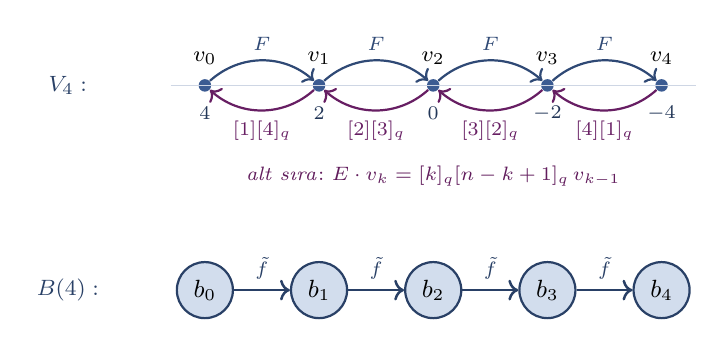
\begin{tikzpicture}[x=1.45cm,y=1cm]
  % --- Agirlik diyagrami V_4 ---
  \node[glabel, accent!70!black] at (-1.2,0) {$V_4:$};
  \foreach \k/\w in {0/4,1/2,2/0,3/-2,4/-4}{
    \node[rdot] (v\k) at (\k,0) {};
    \node[font=\footnotesize] at (\k,0.34) {$v_{\k}$};
    \node[font=\scriptsize, accent!60!black] at (\k,-0.36) {$\w$};
  }
  \draw[accent!25!white, line width=0.6pt] (-0.3,0) -- (4.3,0);
  % F oklari (ustte)
  \foreach \a/\b in {0/1,1/2,2/3,3/4}{
    \draw[->, accent!80!black, line width=0.8pt]
      (v\a) to[bend left=42] node[above, font=\scriptsize] {$F$} (v\b);
  }
  % E oklari (altta), katsayilar [k][n-k+1]
  \foreach \a/\b/\c in {1/0/{[1][4]},2/1/{[2][3]},3/2/{[3][2]},4/3/{[4][1]}}{
    \draw[->, oddsign!75!black, line width=0.8pt]
      (v\a) to[bend left=42] node[below, font=\scriptsize] {$\c_q$} (v\b);
  }
  \node[font=\scriptsize, oddsign!70!black] at (2,-1.15)
    {\emph{alt sıra}: $E\cdot v_k=\qint{k}\qint{n-k+1}\,v_{k-1}$};

  % --- Kristal B(4) ---
  \begin{scope}[yshift=-2.6cm]
    \node[glabel, accent!70!black] at (-1.2,0) {$B(4):$};
    \foreach \k in {0,1,2,3,4}{
      \node[knode] (b\k) at (\k,0) {$b_{\k}$};
    }
    \foreach \a/\b in {0/1,1/2,2/3,3/4}{
      \draw[->, kedge] (b\a) -- node[above, font=\scriptsize] {$\tilde f$} (b\b);
    }
  \end{scope}
\end{tikzpicture}
\caption{\emph{Üstte} $V_4$ temsilinin ağırlık diyagramı: $F$ (mavi) indeksleri
yükseltir, $E$ (mor) $q$-tamsayı katsayılarıyla geri taşır. \emph{Altta} aynı
temsilin $q\to 0$ kristal gölgesi $B(4)$, tek tip $\tilde f$ oklarıyla.}
\label{fig:weight}
\end{figure}

\section{Kristal Tabanlar (Genel Bakış)}

$q \to 0$ limitinde tek tek matris katsayıları ıraksar; ne var ki temsilin
taşıdığı kombinatoryal veri tümüyle kaybolmaz. Kashiwara'nın gözlemi, bu limitte temsile ait bir
\emph{kristal tabanın} --- saf cebirsel verinin kombinatoryal bir iskeletinin ---
hayatta kaldığıdır \cite{Kashiwara,HK}. Bu yüzden kristal tabanı $V_n$'in ``kombinatoryal gölgesi''
olarak düşünmek doğaldır: ağırlık örgüsünün ve operatör eylemlerinin sürekli
katsayıları silinmiş, geriye yalnızca hangi vektörün hangisine bağlandığını
söyleyen yön bilgisi kalmıştır. $\Uq$ için bu gölge $B(n)$, $n+1$ düğüm ve $n$
yönlü kenardan oluşan bir yoldur:
\[
  b_0 \xrightarrow{\tilde{f}} b_1 \xrightarrow{\tilde{f}} \cdots
  \xrightarrow{\tilde{f}} b_n.
\]
Buradaki $\tilde{f}, \tilde{e}$ Kashiwara operatörleri, $F$ ve $E$'nin
$q \to 0$ limitindeki ``kalıntılarıdır''. Bu kombinatoryal yapı sayesinde tensör
çarpımları, karakter formülleri ve dallanma kuralları sürekli hesap yerine
sonlu grafikler üzerinden okunabilir; modern cebirsel kombinatoriğin önemli bir
bölümü bu fikirden beslenir.

\section{Yazılım Mimarisi}

Paketin temel doğrulama deseni, soyut cebirsel eşitlikleri sonlu boyutlu
temsiller üzerinde matris eşitliklerine çevirmektir. Her eşitlik için bir kalıntı
matrisi oluşturulur ve bu matrisin tüm girdileri sembolik olarak sadeleştirilir.
Bu işlem, bir soyut teoremin yerine geçmez; yalnızca seçilen açık temsil
matrislerinde ilgili eşitliğin yeniden üretilebilir biçimde sağlandığını
belgeler. Desen tek tip olduğu için $\Uq$ bağıntılarından Hopf
aksiyomlarına, $R$-matrisi denklemlerinden $GL_q(2|1)$ graded Yang--Baxter
hesabına kadar her doğrulama aynı çekirdek üzerinden yürür; değişen tek şey,
kalıntıyı kuran matrislerin boyutu ve içeriğidir.

Bu yaklaşımın iki pratik dayanağı vardır. Birincisi, temsiller kodda açık bir
veri modeliyle taşınır: her $V_n$ için $E$, $F$, $K$, $K^{-1}$ matrisleri,
$K$-özdeğerleri (\emph{weights}) ve boyut bilgisi tek bir \texttt{Representation}
yapısında toplanır. İkincisi, sıfır kontrolü sayısal değil semboliktir;
\texttt{sympy.simplify} her girdiyi girdi-bazında sadeleştirip $0$'a inip
inmediğine bakar, böylece sonuç belirli bir sayısal $q$ değerine değil formel
$q$ parametresine ilişkin olur \cite{SymPy}. Ayrıca her hesaplamalı iddia, ona karşılık gelen bir
\texttt{pytest} testine bağlanır; dolayısıyla makalede hesaplamalı olarak
doğrulandığı belirtilen her eşitlik, depo klonlandığında yeniden koşturulabilen
somut bir teste karşılık gelir \cite{pytest}.

\texttt{quantum\_group} paketinin modülleri ve sorumlulukları
Tablo~\ref{tab:modules}'te özetlenmiştir.

\begin{table}[h]
\centering
\small
\caption{\texttt{quantum\_group} paketinin modülleri ve sorumlulukları.}
\label{tab:modules}
\begin{tabularx}{\textwidth}{@{}>{\raggedright\arraybackslash}p{0.30\textwidth}X@{}}
\toprule
Modül & Sorumluluk \\
\midrule
\texttt{utils.py} & $q$-tamsayı, $q$-faktöriyel, $q$-binom, klasik limit. \\
\texttt{generators.py} & Sembolik üreteçler $E, F, K, K^{-1}, q$. \\
\texttt{relations.py} & Tanımlayıcı bağıntılar ve matris doğrulaması. \\
\texttt{representations.py} & $V_n$ temsilinin açık matrislerle inşası. \\
\texttt{quantum\_group\_sl2.py} & \texttt{QuantumGroupSL2} cephe sınıfı. \\
\texttt{hopf.py} & $\cop, \eps, S$ ve Hopf aksiyomlarının doğrulaması. \\
\texttt{tensor.py} & $V_m \otimes V_n$ ve Clebsch--Gordan ayrışımı. \\
\texttt{r\_matrix.py} & $R$-matris, QYBE, örgü bağıntısı, Hecke skein. \\
\texttt{supergroup\_gl21.py} & $GL_q(2|1)$ $R$-matrisi, süper permütasyon, graded YBE ve $V^{\otimes n}$ üzerinde $R_{ij}$ yerleşimleri. \\
\texttt{limits.py} & Klasik / genel $q$ / birim kök / kristal limitleri. \\
\texttt{crystal.py} & $B(n)$ kristal grafiği. \\
\texttt{visualization.py} & Ağırlık diyagramı ve kristal grafiği çizimi. \\
\bottomrule
\end{tabularx}
\end{table}

Test paketi (\texttt{tests/}), her modüle karşılık gelen \texttt{pytest} birim
testlerinden oluşur; bu çalışmadaki doğrulama iddiaları bu test dosyalarıyla
eşleştirilmiştir.

\subsection{Yeniden üretilebilirlik}

Depo yapısı üç ana parçadan oluşur: \texttt{quantum\_group/} paket kodunu,
\texttt{tests/} sembolik doğrulama testlerini, \texttt{thesis/} ise LaTeX
kaynağı ile şekil üretim betiklerini içerir. Python 3.10+ ortamında bağımlılıklar
\texttt{python3 -m pip install -r requirements.txt} komutuyla kurulabilir. Tüm matematiksel
kontroller \texttt{python3 -m pytest tests/ -q} ile yeniden çalıştırılır.
Şekiller \texttt{python3 thesis/figures/generate\_figures.py} komutuyla
yeniden üretilebilir; PDF çıktısı \texttt{tectonic thesis/thesis.tex} veya
\texttt{make pdf} hedefiyle derlenir. Depo bağlantısı:
\url{https://github.com/TerekliTahaBerk/quantum-groups}.

\paragraph{Bağıntıların doğrulanması.} Yukarıda anlatılan desenin en yalın
örneği, dört tanımlayıcı bağıntının denetimidir. Her bağıntı $X = Y$ biçiminde
yazılır; kod $V_n$ üzerinde $Z := X - Y$ kalıntı matrisini kurar ve girdilerinin
\texttt{sympy.simplify} altında sıfıra indiğini denetler. Aynı prosedür sembolik
$q$ ile çalıştığından, dört bağıntının da $V_0,\dots,V_4$ üzerinde sağlandığı
tek seferde doğrulanır. Çekirdek mantık şöyledir:

\begin{pythoncode}{Tanımlayıcı bağıntıların sıfır-kalıntı yöntemiyle doğrulanması}
def verify_on_representation(E, F, K, K_inv, q_sym=q):
    I = sp.eye(E.rows)
    # Write each relation as an X - Y residual matrix
    residuals = {
        "R1": K*K_inv - I,
        "R2": K*E*K_inv - q_sym**2 * E,
        "R3": K*F*K_inv - q_sym**(-2) * F,
        "R4": E*F - F*E - (K - K_inv)/(q_sym - q_sym**(-1)),
    }
    # Entrywise simplification: are all entries symbolically zero?
    return {
        name: all(sp.simplify(x) == 0 for x in M)
        for name, M in residuals.items()
    }
\end{pythoncode}

Fonksiyonun döndürdüğü sözlük, her bağıntı için bir doğru/yanlış değeri taşır;
böylece ``hangi bağıntı hangi temsilde sağlandı'' sorusu makine tarafından
yanıtlanabilir bir biçime kavuşur. Bu kod parçasının depo karşılığı
\texttt{quantum\_group/relations.py}, tekrar üretim testi ise
\texttt{tests/test\_relations.py} içindedir. Hopf aksiyomları, $R$-matrisi
denklemleri ve graded YBE de aynı şablonun farklı boyutlardaki uygulamalarıdır.

\paragraph{Boyuttan bağımsızlık.} Bu desenin gücü, kalıntı-matris boyutuna
duyarsız olmasıdır: aynı ``kur ve girdi-bazlı sıfırla'' mantığı $\Uq$
bağıntılarındaki $(n{+}1)\times(n{+}1)$ matrislerden, $GL_q(2|1)$'in
$9\to 27\to 81$ boyutlu tensör kuvvetlerine kadar değişmeden uygulanır. Yüksek
boyutlu yerleşimlerde ($R_{13}$ ve $V^{\otimes 4}$ operatörleri) doğru graded
işaretler, Önerme~\ref{prop:embed}'teki süper-permütasyon konjugasyonuyla
otomatik taşınır; böylece elle hesapta en sık hata yapılan adım --- işaret ve
faktör sıralaması --- kodda yapıya gömülür. Bu, çalışmanın $GL_q(2|1)$
tarafındaki asıl kolaylığının kaynağıdır.

\section{Tensör Çarpımı ve Clebsch--Gordan Ayrışımı}

İlk hesaplamalı katkı, $V_m \otimes V_n$ ayrışımının en yüksek ağırlık
vektörlerini $q$-deforme katsayılarıyla sembolik olarak elde etmektir. Klasik
$\sl_2$ kuramında Clebsch--Gordan formülü
\[
  V_m \otimes V_n \cong V_{m+n} \oplus V_{m+n-2} \oplus \dots \oplus V_{|m-n|}
\]
biçimindedir. Kuantum durumda ayrışımın \emph{kombinatoryal iskeleti} aynen
korunur; değişen, en yüksek ağırlık vektörlerini veren katsayıların artık
$q$'nun rasyonel fonksiyonlarına dönüşmesidir. Bunun mümkün olmasının nedeni,
tensör çarpımı üzerindeki eylemin --- yukarıda vurgulandığı gibi --- $\Uq$'nin
Hopf yapısı, yani eş-çarpımı tarafından belirlenmesidir.

\subsection{Algoritma}

Verilen $V_m, V_n$ için $V_m \otimes V_n$ üzerinde üreteçlerin etkisi,
eş-çarpımdan Kronecker çarpımı ile hesaplanır:
\begin{align*}
  E \cdot (v \otimes w) &= E v \otimes w + K v \otimes E w, \\
  F \cdot (v \otimes w) &= F v \otimes K^{-1} w + v \otimes F w, \\
  K \cdot (v \otimes w) &= K v \otimes K w.
\end{align*}
$V_m \otimes V_n$'nin "$k$-ağırlık altuzayı" K-özdeğeri $q^k$ olan
vektörler ailesidir; her $k = m+n, m+n-2, \dots, |m-n|$ için bu altuzay
incelenir ve $E$'nin çekirdeği bulunur. Çekirdekteki vektör, $V_k$
parçasının en yüksek ağırlık vektörüdür.

\subsection{Hesaplama Sonuçları}

Aşağıdaki ayrışımlar paket tarafından otomatik üretilmiştir.

\paragraph{$V_1 \otimes V_1$.}
\[
  V_1 \otimes V_1 \cong V_2 \oplus V_0.
\]
En yüksek ağırlık vektörleri (baz: $v_0\!\otimes\! v_0,\ v_0\!\otimes\! v_1,\ v_1\!\otimes\! v_0,\ v_1\!\otimes\! v_1$):
\[
  \hwt^{(2)} = (1, 0, 0, 0)^\top, \qquad
  \hwt^{(0)} = \big(0,\ -q^{-1},\ 1,\ 0\big)^\top.
\]
$V_0$ parçasının vektörü, klasik antisimetrik vektör
$(0, -1, 1, 0)/\sqrt{2}$'nin $q$-deforme hâli olup, $-q^{-1}$ katsayısı
$q$-deformasyonun cebirsel parmak izidir.

\paragraph{$V_2 \otimes V_2$.}
\[
  V_2 \otimes V_2 \cong V_4 \oplus V_2 \oplus V_0.
\]
$V_0$ singleti (baz $v_i \otimes v_j$, $i,j \in \{0,1,2\}$ üzerinde):
\[
  \hwt^{(0)} = (0, 0, q^{-2}, 0, -1, 0, 1, 0, 0)^\top.
\]
Klasik limitte $q \to 1$: $(0,0,1,0,-1,0,1,0,0)^\top$, klasik
Clebsch--Gordan ile uyumludur.

\paragraph{$V_3 \otimes V_2$.}
\[
  V_3 \otimes V_2 \cong V_5 \oplus V_3 \oplus V_1.
\]
$V_3$ parçasının en yüksek ağırlık vektörü, sıfırdan farklı iki konumda
\[
  -\frac{q^4 + q^2 + 1}{q^6 + q^4} \quad\text{ve}\quad 1
\]
katsayılarına sahiptir. $q \to 1$ limitinde $-3/2$ ve $1$, yani
$\binom{3}{1}/\binom{2}{0}$ tipi klasik Clebsch--Gordan oranını verir.

\subsection{Doğrulama}

Üretilen her aday vektör $v$'nin gerçekten bir en yüksek ağırlık vektörü olduğu
iki koşulla denetlenir:
\[
  E \cdot v = 0, \qquad K \cdot v = q^k v.
\]
Bu iki eşitlik seçilen temsiller üzerinde sembolik olarak doğrulanmıştır
(bkz.\ \path{tests/test_tensor.py}, \path{test_highest_weight_vectors_killed_by_E}).
Buna ek olarak, $\cop$ üzerinden taşınan eylemle $V_m \otimes V_n$'in dört
tanımlayıcı bağıntıyı (R1)--(R4) sağladığı da temsil düzeyinde doğrulanmıştır
(\path{test_tensor_satisfies_relations}); yani tensör çarpımı yalnızca bir
vektör uzayı değil, gerçek bir $\Uq$-modülüdür.

\section{R-Matrisi ve Yang--Baxter Denklemi}

Bu bölümdeki hesap, $\Uq$ için $R$-matrisini kurup kuantum Yang--Baxter
denklemini ve buna eşlik eden örgü/Hecke bağıntılarını sembolik matris düzeyinde
kontrol eder. Literatürde evrensel $R$-matrisi ve örgülü monoidal kategori
yorumu standarttır \cite{Drinfeld,Jimbo,Kassel}; burada yapılan iş, bu yapının
$V_1 \otimes V_1$ üzerindeki açık matris modelini kodlayıp kalıntı testiyle
izlenebilir hâle getirmektir. $\Uq$ söz konusu olduğunda bu eleman,
$V_1 \otimes V_1$ üzerinde şu $4 \times 4$ matrise iner:
\begin{equation}\label{eq:R}
  R = \begin{pmatrix}
    q & 0 & 0 & 0 \\
    0 & 1 & q - q^{-1} & 0 \\
    0 & 0 & 1 & 0 \\
    0 & 0 & 0 & q
  \end{pmatrix},
\end{equation}
baz sıralaması $v_0\!\otimes\! v_0,\ v_0\!\otimes\! v_1,\ v_1\!\otimes\! v_0,\ v_1\!\otimes\! v_1$.
Bu matrisin ve örgülü eşi $\Rcheck=\tau R$'nin yapısı, paket tarafından üretilen
Şekil~\ref{fig:rsl2}'de verilmiştir; tek köşegen-dışı terim $q-q^{-1}$,
deformasyonun izini taşır.

\begin{figure}[h]
\centering
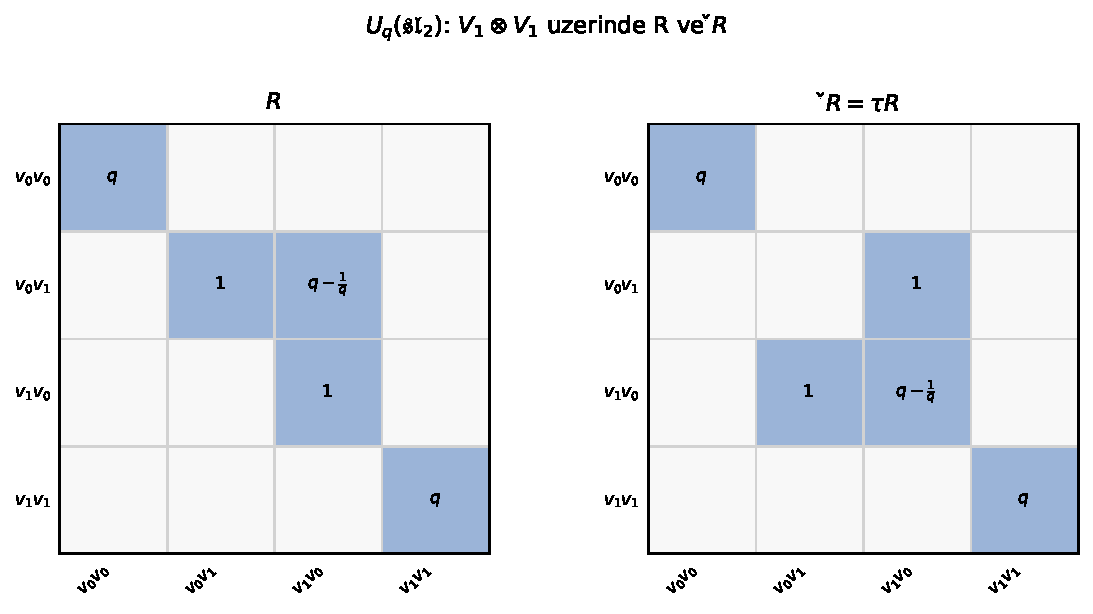
\includegraphics[width=0.82\textwidth]{R_sl2_V1.pdf}
\caption{$V_1\otimes V_1$ üzerinde Drinfeld $R$-matrisi ve örgülü $\Rcheck=\tau R$.
Renkli hücreler sıfırdan farklı girdileri, içlerindeki ifadeler ise girdinin
değerini gösterir (doğrudan \texttt{R\_matrix\_V1} / \texttt{R\_check\_V1}
çıktısı).}
\label{fig:rsl2}
\end{figure}

\subsection{Kuantum Yang--Baxter Denklemi}

$V_1^{\otimes 3}$ üzerinde $R$-matris denklemi şudur:
\begin{equation}\label{eq:QYBE}
  R_{12} R_{13} R_{23} = R_{23} R_{13} R_{12},
\end{equation}
burada $R_{ij}$, üçlü çarpımın $i$ ve $j$. faktörlerine $R$ olarak etki edip
kalan faktörde özdeşlik gibi davranan $8\times 8$ operatördür. Bu indislerin
önemi yüzeysel değildir: $R_{12}$ ile $R_{23}$ komşu faktörlere ($\otimes I$
ya da $I\otimes$ biçiminde) doğrudan yerleştirilebilirken, $R_{13}$ \emph{komşu
olmayan} birinci ve üçüncü faktörlere etki eder ve ancak araya bir takas
operatörü sokularak kurulabilir. Yang--Baxter denklemi, bu üç yerleşimin
çarpım sırasının (``önce 12 sonra 23'' ile tersi) aynı operatörü vermesini ister;
geometrik olarak bu, Şekil~\ref{fig:ybe}'deki üç doğrunun ortasındaki kesişimden
ikinci doğrunun hangi yönden geçtiğinin --- yani örülme sırasının --- sonucu
değiştirmemesi koşuludur.

\begin{figure}[h]
\centering
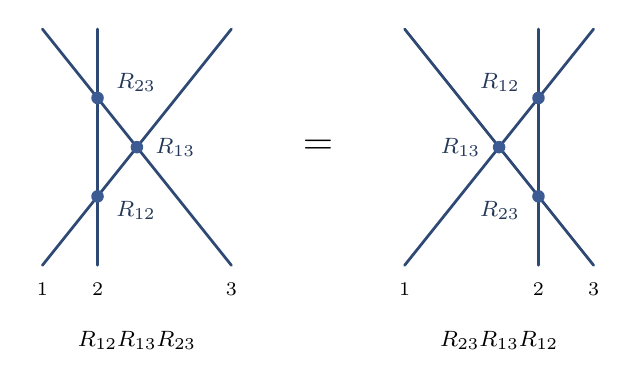
\begin{tikzpicture}[scale=1.0,line cap=round]
  % ====== SOL: ikinci dogru solda ======
  \begin{scope}
    \draw[strand] (0,0) -- (2.4,3);          % dogru 1
    \draw[strand] (0.7,0) -- (0.7,3);         % dogru 2 (solda)
    \draw[strand] (2.4,0) -- (0,3);           % dogru 3
    \node[rdot] at (0.7,0.875) {}; \node[glabel,right=1pt] at (0.78,0.7) {$R_{12}$};
    \node[rdot] at (1.2,1.5)   {}; \node[glabel,right=1pt] at (1.28,1.5) {$R_{13}$};
    \node[rdot] at (0.7,2.125) {}; \node[glabel,right=1pt] at (0.78,2.32) {$R_{23}$};
    \node[font=\scriptsize] at (0,-0.3){1}; \node[font=\scriptsize] at (0.7,-0.3){2};
    \node[font=\scriptsize] at (2.4,-0.3){3};
    \node[font=\footnotesize] at (1.2,-0.95) {$R_{12}R_{13}R_{23}$};
  \end{scope}
  % ====== Esittir ======
  \node[font=\Large] at (3.5,1.5) {$=$};
  % ====== SAG: ikinci dogru sagda (ayna) ======
  \begin{scope}[xshift=4.6cm]
    \draw[strand] (0,0) -- (2.4,3);
    \draw[strand] (1.7,0) -- (1.7,3);         % dogru 2 (sagda)
    \draw[strand] (2.4,0) -- (0,3);
    \node[rdot] at (1.7,2.125) {}; \node[glabel,left=1pt] at (1.62,2.32) {$R_{12}$};
    \node[rdot] at (1.2,1.5)   {}; \node[glabel,left=1pt] at (1.12,1.5) {$R_{13}$};
    \node[rdot] at (1.7,0.875) {}; \node[glabel,left=1pt] at (1.62,0.7) {$R_{23}$};
    \node[font=\scriptsize] at (0,-0.3){1}; \node[font=\scriptsize] at (1.7,-0.3){2};
    \node[font=\scriptsize] at (2.4,-0.3){3};
    \node[font=\footnotesize] at (1.2,-0.95) {$R_{23}R_{13}R_{12}$};
  \end{scope}
\end{tikzpicture}
\caption{Kuantum Yang--Baxter denkleminin doğru-diyagramı. Üç doğru ikişerli
kesişir; her kesişim bir $R_{ij}$ operatörüdür. İkinci doğruyu $R_{13}$
kesişiminin soluna ya da sağına kaydırmak operatörü değiştirmez:
$R_{12}R_{13}R_{23}=R_{23}R_{13}R_{12}$.}
\label{fig:ybe}
\end{figure}

\begin{theorem}[Temsil düzeyinde hesaplamalı doğrulama]\label{thm:QYBE}
\eqref{eq:R} ile verilen $R$-matrisi \eqref{eq:QYBE} kuantum
Yang--Baxter denklemine karşılık gelen kalıntıyı $V_1^{\otimes 3}$ üzerinde
sıfırlar. Başka bir ifadeyle
$R_{12} R_{13} R_{23} - R_{23} R_{13} R_{12}$ kalıntı matrisi, sembolik $q$
üzerinde $8 \times 8$ sıfır matrise sadeleşir.
\end{theorem}

\begin{proof}[Doğrulama]
Burada $R_{12}=R\otimes\id$ ve $R_{23}=\id\otimes R$ doğrudandır; uzak yerleşim
$R_{13}$ ise takas matrisi $\tau$ ile konjuge edilerek kurulur. Çekirdek
hesap şudur:
\begin{pythoncode}{QYBE kalıntısı ve $R_{13}$'ün takasla inşası}
def qybe_residual(R):
    d = int(sp.sqrt(R.rows))
    I = sp.eye(d)
    R12 = _kron(R, I)
    R23 = _kron(I, R)
    # R13 = (id (x) tau) (R (x) id) (id (x) tau)
    P23 = _kron(I, swap_matrix(d))
    R13 = sp.simplify(P23 * R12 * P23)
    return sp.simplify(R12 * R13 * R23 - R23 * R13 * R12)
\end{pythoncode}
\texttt{sympy.simplify} sonucun $64$ girdisini de sıfıra indirir; dolayısıyla
seçilen açık temsil üzerinde kalıntı $8\times 8$ sıfır matristir. (Kod: \path{quantum_group/r_matrix.py},
\path{qybe_residual}; test \path{tests/test_r_matrix.py}, \path{test_R_satisfies_qybe}.)
\end{proof}

\subsection{Örgülü R-Matrisi ve Hecke Skein Bağıntısı}

$R$'nin önüne takas operatörü $\tau$ eklenerek tanımlanan
$\check R := \tau \circ R$, \emph{örgülü $R$-matrisi} adını alır. Bu küçük
değişiklik kavramsal olarak önemlidir: $R$ Yang--Baxter denklemini ``düz''
biçimde sağlarken, $\check R$ örgü grubu $B_n$'in bir temsilini doğrudan üretir;
yani her tensör çarpanı bir ipliğe, $\check R$ ise iki komşu ipliğin
çaprazlamasına karşılık gelir.

\begin{proposition}[Örgü bağıntısının hesaplamalı doğrulaması]\label{thm:braid}
$\check R$ aşağıdakini sağlar:
\[
  \check R_{12} \check R_{23} \check R_{12} = \check R_{23} \check R_{12} \check R_{23}.
\]
\end{proposition}

Bu, $B_3$ örgü grubunun $\sigma_1\sigma_2\sigma_1 = \sigma_2\sigma_1\sigma_2$
üreteç ilişkisinin matris karşılığıdır. Test karşılığı
\texttt{tests/test\_r\_matrix.py::test\_R\_check\_satisfies\_braid\_relation}
adlı kontroldür. Üstelik $\check R$ keyfi bir örgü temsili değildir; sağladığı
ikinci dereceden bir özdeşlik, onu Hecke cebrine bağlar \cite{Jones,Kassel}:

\begin{proposition}[Hecke skein bağıntısının hesaplamalı doğrulaması]\label{thm:hecke}
$\check R$ aşağıdaki kuadratik bağıntıyı sağlar:
\[
  \check R - \check R^{-1} = (q - q^{-1})\, I_4.
\]
\end{proposition}

\begin{proof}[Doğrulama]
$\check R$'nin $4 \times 4$ açık matrisini ve $\check R^{-1}$'i SymPy
ile hesaplayıp farkı sadeleştirdiğimizde tam olarak
$(q - q^{-1}) I_4$ elde ederiz. Test
\texttt{tests/test\_r\_matrix.py::test\_jones\_skein}.
\end{proof}

\subsection{Spektral Ayrışma ve Clebsch--Gordan ile Bağlantı}

\begin{proposition}\label{prop:eigs}
$\check R$'nin $V_1 \otimes V_1$ üzerindeki özdeğerleri ve çoklukları:
\[
  \mathrm{spec}(\check R) = \{q^{(3)},\ -q^{-1\,(1)}\}.
\]
\end{proposition}

Bu spektrum, $V_1 \otimes V_1 = V_2 \oplus V_0$ Clebsch--Gordan ayrışımıyla
birebir örtüşür (Şekil~\ref{fig:spec}): $q$ özdeğerinin üç-katlı özuzayı simetrik
parça $V_2$'ye, $-q^{-1}$ özdeğerinin tek-katlı özuzayı ise antisimetrik singlet
$V_0$'a karşılık gelir. Topolojik okuması da nettir: $q$ ``ışınımsız geçiş'',
$-q^{-1}$ ise ``işaret değiştiren yarım-tur'' ile ilişkilenir.

\begin{figure}[h]
\centering
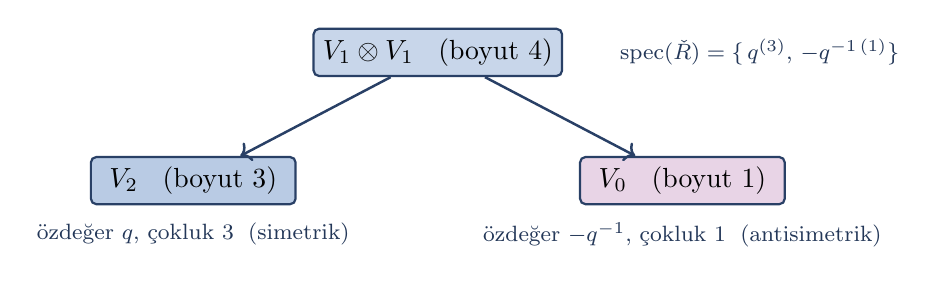
\begin{tikzpicture}[node distance=8mm]
  \node[rbox, minimum width=30mm] (vv) {$V_1\otimes V_1$\;\; (boyut 4)};
  \node[rbox, fill=accentsoft!70, minimum width=26mm, below left=10mm and 2mm of vv] (v2)
    {$V_2$\;\; (boyut 3)};
  \node[rbox, fill=oddsign!20, minimum width=26mm, below right=10mm and 2mm of vv] (v0)
    {$V_0$\;\; (boyut 1)};
  \draw[kedge,->] (vv) -- (v2);
  \draw[kedge,->] (vv) -- (v0);
  \node[glabel, below=1mm of v2] {özdeğer $q$, çokluk 3 \;(simetrik)};
  \node[glabel, below=1mm of v0] {özdeğer $-q^{-1}$, çokluk 1 \;(antisimetrik)};
  \node[glabel, accent!60!black, right=6mm of vv, align=left]
    {$\mathrm{spec}(\Rcheck)=\{\,q^{(3)},\,-q^{-1\,(1)}\}$};
\end{tikzpicture}
\caption{Örgülü $\Rcheck$'nin spektral ayrışması, $V_1\otimes V_1=V_2\oplus V_0$
Clebsch--Gordan ayrışımıyla aynıdır. Özdeğer çoklukları doğrudan alt-temsil
boyutlarını verir (\texttt{R\_check\_eigenvalues}).}
\label{fig:spec}
\end{figure}

\subsection{Düğüm Değişmezleriyle Bağlantı (İleri Görü)}

Hecke skein bağıntısı, $\check R$ ile üretilen $B_n$ temsilinin Hecke cebri
$H_n(q)$ üzerinden çarpanlandığını gösteren standart yola bağlanır. Uygun bir
Markov izi eklendiğinde bu çerçeve $\sl_2$ tipindeki Jones polinomu ile
ilişkilidir \cite{Jones}. Bu makalede Jones polinomunun kendisi
hesaplanmamıştır; yalnızca ona giden iki matris düzeyindeki basamak --- örgü
bağıntısı ve Hecke özdeşliği (Önerme~\ref{thm:braid} ve~\ref{thm:hecke}) ---
seçilen $V_1\otimes V_1$ modeli üzerinde doğrulanmıştır.

\section{$GL_q(2|1)$ için Graded Yang--Baxter Doğrulaması}

Makalenin ayırt edici hesaplamalı katkısı bu bölümdedir: kuantum süpergrup
$GL_q(2|1)$ için literatürde verilen $R$-matrisi, seçilen baz sıralaması ve
parite konvansiyonu altında graded Yang--Baxter kalıntısına yerleştirilir.
Amaç yeni bir RTT inşası vermek değil, literatürdeki $9\times 9$ matrisin
$27\times 27$ kalıntı testiyle yeniden üretilebilir biçimde kontrol edilmesidir.

\subsection{Motivasyon}

Salih Çelik ve Sultan A.\ Çelik \cite{CelikGL21}, $GL_q(2|1)$ kuantum süpergrubunu
$V=\mathbb{C}^{2|1}$ süper vektör uzayı üzerindeki bir $R$-matrisinden RTT
yöntemiyle inşa eder. Bu makaledeki hesap, o çalışmada verilen $9\times 9$
$R$-matrisini bağımsız olarak kodlar ve graded Yang--Baxter eşitliğine ait
kalıntının tüm girdilerde sıfıra sadeleştiğini denetler.

Bu doğrulamanın el ile yapılması zahmetlidir: denklem $27\times 27$ matrislerin
çarpımına dayanır ve uzun, tekrarlı yapısı nedeniyle işaret/sıralama hatalarına
açıktır. Dahası --- birazdan görüleceği gibi --- graded yapı, sıradan bir
matris hesabının ötesinde parite bilgisinin doğru taşınmasını da gerektirir. Bu
iki neden, hesabı açık baz, açık parite ve açık süper permütasyon matrisiyle
Python/SymPy üzerinde modellemeyi doğal kılar \cite{SymPy}.

Baz sıralaması $e_1e_1,\,e_1e_2,\,e_1e_3,\,e_2e_1,\,e_2e_2,\,e_2e_3,\,
e_3e_1,\,e_3e_2,\,e_3e_3$ (kısaca $e_ie_j:=e_i\otimes e_j$) alındığında, kodlanan
$9\times 9$ $R$-matrisi şudur:
\begin{equation}\label{eq:Rgl21}
\setlength{\arraycolsep}{3.2pt}
R=\begin{pmatrix}
1 & 0    & 0 & 0      & 0 & 0    & 0      & 0      & 0\\
0 & q^2  & 0 & 1-q^2  & 0 & 0    & 0      & 0      & 0\\
0 & 0    & q & 0      & 0 & 0    & 1-q^2  & 0      & 0\\
0 & 0    & 0 & 1      & 0 & 0    & 0      & 0      & 0\\
0 & 0    & 0 & 0      & 1 & 0    & 0      & 0      & 0\\
0 & 0    & 0 & 0      & 0 & q    & 0      & 1-q^2  & 0\\
0 & 0    & 0 & 0      & 0 & 0    & q      & 0      & 0\\
0 & 0    & 0 & 0      & 0 & 0    & 0      & q      & 0\\
0 & 0    & 0 & 0      & 0 & 0    & 0      & 0      & q^2
\end{pmatrix}.
\end{equation}
Girdilerin yalnızca dört farklı türü ($1,\,q,\,q^2,\,1-q^2$) ve seyrek yerleşimi,
paketin ürettiği Şekil~\ref{fig:rgl21}'de renk kodlu olarak görülebilir.

\begin{figure}[h]
\centering
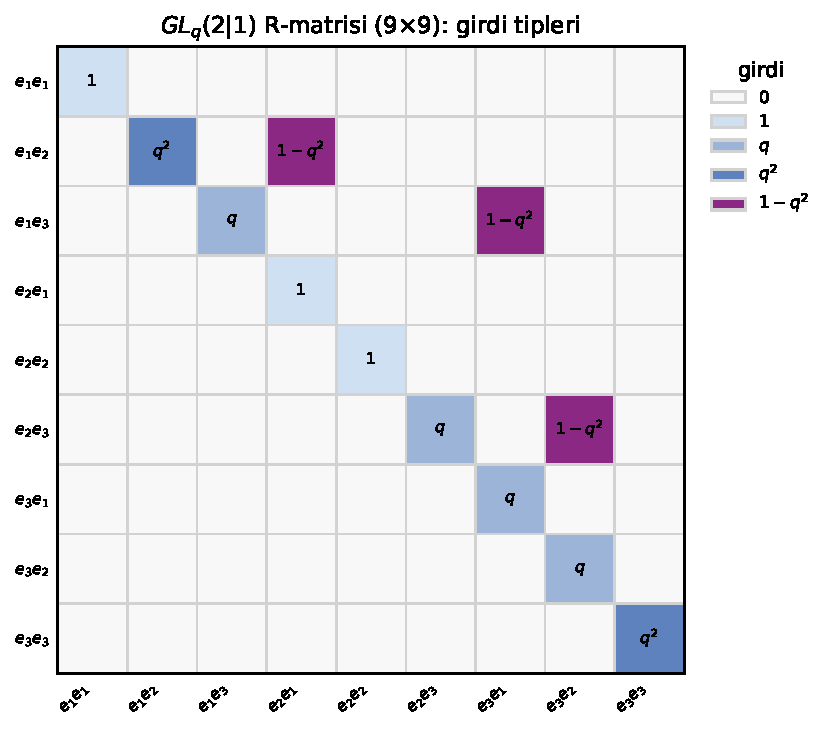
\includegraphics[width=0.74\textwidth]{R_gl21_structure.pdf}
\caption{\eqref{eq:Rgl21} R-matrisinin girdi-tipi haritası (\texttt{R\_matrix\_GLq21}
çıktısı). Köşegen $q$/$q^2$ terimleri ile köşegen-dışı $1-q^2$ ``karışım''
terimleri açıkça ayrışır; bu seyreklik, $27\times 27$ ve $81\times 81$
yerleşimlerin neden hâlâ hesaplanabilir kaldığını da açıklar.}
\label{fig:rgl21}
\end{figure}

\subsection{Graded Yapı ve Süper Permütasyon}

Süper vektör uzayı $V=\mathbb{C}^{2|1}$'in baz vektörleri parite (derece)
taşır:
\[
p(e_1)=0,\qquad p(e_2)=0,\qquad p(e_3)=1,
\]
yani $e_1,e_2$ çift, $e_3$ tektir. Graded ortamda iki faktörün yer değiştirmesi,
klasik takasla aynı olamaz: süper cebirde iki tek (odd) nesne yer değiştirirken
Koszul işaret kuralı gereği bir eksi işareti ortaya çıkar. Bu, $V\otimes V$
üzerindeki \emph{süper permütasyon} matrisiyle kodlanır:
\[
P(e_i\otimes e_j)=(-1)^{p(e_i)p(e_j)}\,e_j\otimes e_i.
\]
Dolayısıyla $P$, klasik permütasyon matrisinden yalnızca tek--tek (odd--odd)
bileşendeki işaret değişimiyle ayrılır. Bu küçük görünen ayrıntı belirleyicidir:
$R_{13}$ operatörü süper permütasyon yardımıyla kurulduğundan, işaret yanlış
modellenirse $R_{13}$ ve onunla birlikte tüm graded Yang--Baxter hesabı
matematiksel olarak anlamını yitirir. Kod, bu parite bilgisini doğrudan matris
düzeyine taşır; bu fonksiyonun involüsyon ve $P[8,8]=-1$ kontrolleri
\texttt{tests/test\_supergroup\_gl21.py} içinde yer alır:

\begin{pythoncode}{$V \otimes V$ üzerinde süper permütasyon matrisi}
def super_permutation_matrix(parity):
    d = len(parity)
    P = sp.zeros(d*d, d*d)
    for i in range(d):
        for j in range(d):
            # Koszul sign: -1 only on the odd-odd component
            sign = -1 if parity[i] and parity[j] else 1
            P[j*d + i, i*d + j] = sign
    return P
\end{pythoncode}

$GL_q(2|1)$ için \texttt{parity}$=[0,0,1]$ verildiğinden eksi işareti yalnızca
$e_3\otimes e_3$ bileşeninde, yani $P[8,8]=-1$ girdisinde belirir; kalan tüm
girdiler klasik takasla aynıdır (Şekil~\ref{fig:superperm}).

\begin{figure}[h]
\centering
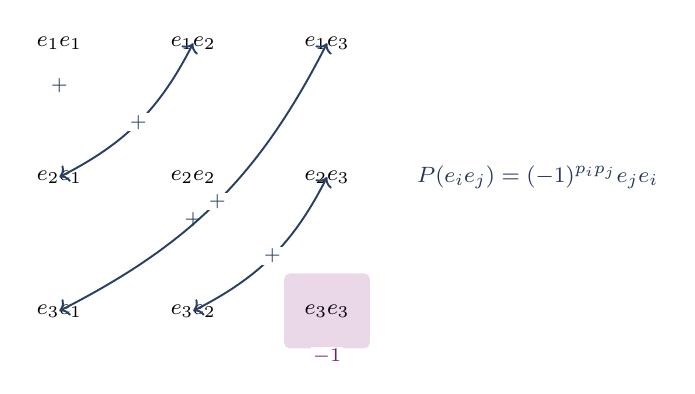
\begin{tikzpicture}[x=1.7cm,y=1.7cm]
  % 3x3 baz izgarasi: hucre (i,j) -> e_i e_j
  \foreach \i in {1,2,3}{
    \foreach \j in {1,2,3}{
      \coordinate (c\i\j) at (\j, -\i);
    }
  }
  % odd-odd hucresi (3,3) vurgulu
  \fill[oddsign!18, rounded corners=2pt] (3-0.32,-3-0.28) rectangle (3+0.32,-3+0.28);
  \foreach \i in {1,2,3}{
    \foreach \j in {1,2,3}{
      \node[font=\footnotesize] at (c\i\j) {$e_{\i}e_{\j}$};
    }
  }
  % kosegen-disi takas oklari (+1)
  \foreach \i/\j in {1/2,1/3,2/3}{
    \draw[<->, accent!70!black, line width=0.7pt]
      (c\i\j) to[bend left=18] node[font=\scriptsize, fill=white, inner sep=0.6pt] {$+$} (c\j\i);
  }
  % kosegen sabit (isaret)
  \node[font=\scriptsize, accent!60!black] at (1+0.0,-1-0.32) {$+$};
  \node[font=\scriptsize, accent!60!black] at (2+0.0,-2-0.32) {$+$};
  \node[font=\scriptsize, oddsign!80!black, fill=white, inner sep=0.6pt] at (3,-3-0.34) {$-1$};
  \node[glabel, accent!60!black, anchor=west] at (3.6,-2)
    {$P(e_ie_j)=(-1)^{p_ip_j}e_je_i$};
\end{tikzpicture}
\caption{Süper permütasyon $P$, $V\otimes V$ bazı üzerinde bir takas: köşegen-dışı
çiftler işaretsiz ($+$) yer değiştirir, köşegen sabit kalır; tek istisna
odd--odd köşesi $e_3e_3$'tür ($-1$, vurgulu). Klasik takastan tek fark budur.}
\label{fig:superperm}
\end{figure}

\subsection{$R_{12}, R_{13}, R_{23}$ Yerleşimleri}

Makaledeki $R$-matrisi $V\otimes V$ üzerinde etki eden $9\times 9$ bir
operatördür. Üçlü çarpım $V\otimes V\otimes V$ üzerinde komşu faktör
yerleşimleri doğrudandır:
\[
R_{12}=R\otimes I_3,\qquad R_{23}=I_3\otimes R.
\]
Komşu olmayan birinci ve üçüncü faktöre etki eden $R_{13}$ ise ancak süper
permütasyonla eşlenerek kurulabilir:
\[
R_{13}=(P\otimes I_3)\,R_{23}\,(P\otimes I_3).
\]
İşte parite bilgisinin hesaba sızdığı yer tam da budur: $R_{13}$, $R_{23}$'ün
süper permütasyonla ``iki kez döndürülmüş'' hâlidir ve $P$'deki tek eksi işaret
doğrudan bu operatöre geçer. Şekil~\ref{fig:place} bu üç yerleşimi iplik
diyagramı olarak karşılaştırır: $R_{12}$ ve $R_{23}$ komşu ipliklere doğrudan
oturur, $R_{13}$ ise 1.\ ve 3.\ iplikleri süper permütasyonla komşulaştırıp
$R$'yi uygulayıp tekrar açan bir konjugasyonla kurulur.

\begin{figure}[h]
\centering
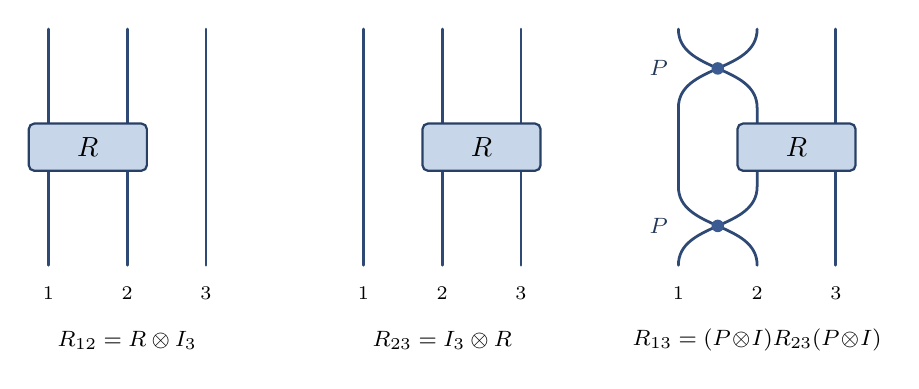
\begin{tikzpicture}[x=1cm,y=1cm,line cap=round]
  % ---- R12 ----
  \begin{scope}
    \draw[strand] (0,0)--(0,3); \draw[strand] (1,0)--(1,3); \draw[strand] (2,0)--(2,3);
    \node[rbox, minimum width=15mm] at (0.5,1.5) {$R$};
    \foreach \k/\x in {1/0,2/1,3/2}{\node[font=\scriptsize] at (\x,-0.35){\k};}
    \node[font=\footnotesize] at (1,-0.95) {$R_{12}=R\otimes I_3$};
  \end{scope}
  % ---- R23 ----
  \begin{scope}[xshift=4cm]
    \draw[strand] (0,0)--(0,3); \draw[strand] (1,0)--(1,3); \draw[strand] (2,0)--(2,3);
    \node[rbox, minimum width=15mm] at (1.5,1.5) {$R$};
    \foreach \k/\x in {1/0,2/1,3/2}{\node[font=\scriptsize] at (\x,-0.35){\k};}
    \node[font=\footnotesize] at (1,-0.95) {$R_{23}=I_3\otimes R$};
  \end{scope}
  % ---- R13 (konjugasyon) ----
  \begin{scope}[xshift=8cm]
    % strand A: 0 -> swap -> pos1 -> swap back -> 0
    \draw[strand] (0,0) to[out=90,in=-90] (1,1) -- (1,2) to[out=90,in=-90] (0,3);
    % strand B: 1 -> 0 -> 1
    \draw[strand] (1,0) to[out=90,in=-90] (0,1) -- (0,2) to[out=90,in=-90] (1,3);
    % strand C: 2 duz
    \draw[strand] (2,0) -- (2,3);
    % P kesisimleri
    \node[rdot] at (0.5,0.5){}; \node[rdot] at (0.5,2.5){};
    \node[glabel] at (-0.25,0.5){$P$}; \node[glabel] at (-0.25,2.5){$P$};
    % R kutusu orta bolgede pos2(=x1) ve pos3(=x2) uzerinde
    \node[rbox, minimum width=15mm] at (1.5,1.5) {$R$};
    \foreach \k/\x in {1/0,2/1,3/2}{\node[font=\scriptsize] at (\x,-0.35){\k};}
    \node[font=\footnotesize] at (1,-0.95) {$R_{13}=(P\!\otimes\! I)R_{23}(P\!\otimes\! I)$};
  \end{scope}
\end{tikzpicture}
\caption{Üç faktörlü uzayda $R_{ij}$ yerleşimleri. Komşu yerleşimler ($R_{12},R_{23}$)
basit Kronecker gömmeleridir; uzak yerleşim $R_{13}$ ise süper permütasyon $P$
ile konjugasyon gerektirir --- elle takibi en zor olan, bu çalışmada
otomatikleştirilen adım.}
\label{fig:place}
\end{figure}

Bu fikir tek bir yerleşime özgü değildir. Pakette, $R$'yi herhangi bir
$V^{\otimes n}$ uzayında istenen $(i,j)$ faktör çiftine taşıyan genel bir gömme
fonksiyonu tanımlıdır.

\begin{proposition}[Konjugasyonla genel yerleşim]\label{prop:embed}
$d=\dim V$ ve $S_k$, $k$ ile $k{+}1$ faktörlerini değiş-tokuş eden komşu graded
takas operatörü olsun ($S_k=I^{\otimes k}\otimes P\otimes I^{\otimes(n-k-2)}$).
$i<j$ için $V^{\otimes n}$ üzerindeki $R_{i,j}$ operatörü, komşu yerleşim
$R_{i,i+1}=I^{\otimes i}\otimes R\otimes I^{\otimes(n-i-2)}$'in ardışık
konjugasyonuyla elde edilir:
\[
R_{i,j}=S_{j-1}\cdots S_{i+1}\,R_{i,i+1}\,S_{i+1}\cdots S_{j-1}.
\]
Bu konjugasyon graded işaretleri doğru taşır; $j=i+1$ için ifade basit Kronecker
gömmesine indirgenir.
\end{proposition}

Bu önermenin kod karşılığı doğrudan ve test edilebilirdir; $R_{13}$'ün sıradan
takasla değil süper permütasyonla kurulduğu yine
\texttt{tests/test\_supergroup\_gl21.py} içinde ayrıca denetlenir:

\begin{pythoncode}{$R$-matrisini $V^{\otimes n}$ içinde $(i,j)$ faktörlerine gömme}
def embed_R_in_tensor_power(R, positions, tensor_power, parity):
    i, j = positions                       # zero-based indices, i < j
    d, n = len(parity), tensor_power
    # Adjacent placement R_{i, i+1}
    op = _kron_list([_eye_pow(d, i), R, _eye_pow(d, n - i - 2)])
    # Move the second index from i+1 to j by conjugation (graded swap)
    for k in range(i + 1, j):
        S_k = _adjacent_swap(parity, n, k)
        op = S_k * op * S_k
    return op
\end{pythoncode}

$V\otimes V\otimes V$ için $(i,j)=(0,2)$ seçilince bu fonksiyon yukarıdaki
$R_{13}$ formülünü birebir yeniden üretir; $V^{\otimes 4}$'te ise altı
yerleşimin hepsi aynı çağrıyla otomatik kurulur.

\subsection{Sıfır-Kalıntı Yöntemi}

Graded Yang--Baxter denklemi yine
\[
R_{12}R_{13}R_{23}=R_{23}R_{13}R_{12}
\]
biçimindedir. Önceki bölümlerle aynı şablon izlenerek kalıntı matrisi
\[
Y(q)=R_{12}R_{13}R_{23}-R_{23}R_{13}R_{12}
\]
kurulur; bu $27\times 27$ boyutlu bir matristir. SymPy ile yapılan girdi-bazlı
sadeleştirme,
\[
Y(q)_{ij}=0,\qquad 1\leq i,j\leq 27,
\]
yani matrisin tamamının sıfır olduğunu verir. Hesabın çekirdeği şudur:

\begin{pythoncode}{$GL_q(2|1)$ için graded Yang--Baxter kalıntısı}
def graded_yang_baxter_residual_GLq21(q_sym=q):
    # GL_q(2|1) graded Yang-Baxter residual matrix (27x27)
    R12 = R12_GLq21(q_sym)
    R13 = R13_GLq21(q_sym)   # built with the super-permutation
    R23 = R23_GLq21(q_sym)
    return R12*R13*R23 - R23*R13*R12

def graded_yang_baxter_holds_GLq21(q_sym=q):
    Y = graded_yang_baxter_residual_GLq21(q_sym)
    # Are all 27x27 entries symbolically zero?
    return all(sp.simplify(x) == 0 for x in Y)
\end{pythoncode}

Bu fonksiyon $27\times 27$ kalıntıyı oluşturur ve her girdiyi sembolik olarak
sıfıra indirger; tekrar üretim testi
\texttt{tests/test\_supergroup\_gl21.py::test\_graded\_yang\_baxter\_holds\_symbolically}
adlı kontroldür. Sonuç Şekil~\ref{fig:ybe27}'de görselleştirilmiştir: eşitliğin
iki tarafı --- $R_{12}R_{13}R_{23}$ ve $R_{23}R_{13}R_{12}$ --- tıpatıp aynı
sıfır-olmayan örüntüye sahiptir (her birinde $729$ girdiden $58$'i sıfırdan
farklı), farkları $Y(q)$ ise tümüyle boştur. Böylece seçilen baz sıralaması ve
$p=(0,0,1)$ parite konvansiyonu altında graded Yang--Baxter eşitliğinin matris
girdileri düzeyinde sağlandığı hem sembolik hem görsel olarak doğrulanır.

\begin{figure}[h]
\centering
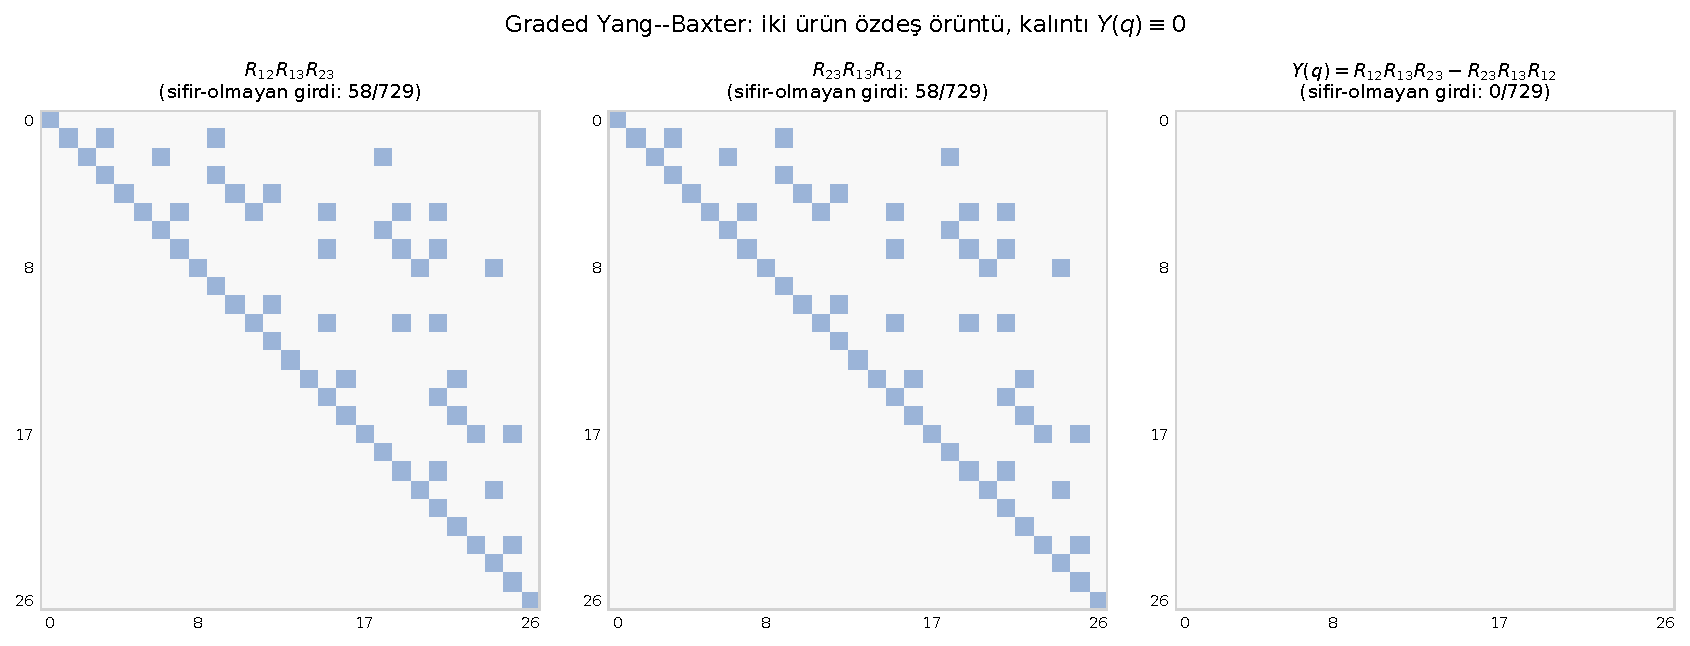
\includegraphics[width=\textwidth]{ybe_products_27.pdf}
\caption{Graded Yang--Baxter denkleminin iki tarafının $27\times 27$
sıfır-olmayan örüntüleri özdeştir; kalıntı $Y(q)=R_{12}R_{13}R_{23}-
R_{23}R_{13}R_{12}$ tüm $729$ girdide sıfırdır
(\texttt{graded\_yang\_baxter\_residual\_GLq21}).}
\label{fig:ybe27}
\end{figure}

\subsection{Dört Faktörlü Genişleme}

Yöntemin tek bir denkleme bağlı kalmadığını göstermek için, $R$-matrisinin
$V^{\otimes n}$ üzerine genel yerleşimini üreten bir fonksiyon da yazılmıştır.
Örneğin $V^{\otimes 4}$ üzerinde
\[
R_{12}, R_{13}, R_{14}, R_{23}, R_{24}, R_{34}
\]
operatörleri $81\times 81$ matrisler olarak elde edilebilir. Bu boyut tesadüfi
değildir: süpergrup hesapları hızla büyür ($3^3=27$, $3^4=81$) ve elle takibi
neredeyse olanaksız hâle gelir; sembolik altyapı ise Önerme~\ref{prop:embed}'in
şablonunu boyuttan bağımsız biçimde uygular. $V^{\otimes 4}$'ün altı yerleşimi
ve aralarındaki ilişkiler, $K_4$ tam grafiği üzerinden okunabilir
(Şekil~\ref{fig:k4}): grafiğin altı kenarı altı $R_{ij}$ operatörüne, dört
üçgeni dört lokal Yang--Baxter kontrolüne, ayrık kenar çifti ise uzak
komütativiteye karşılık gelir. Bu sayede hem uzak komütativite
\[
R_{12}R_{34}=R_{34}R_{12}
\]
hem de dört ayrı üçlü altblok için lokal graded Yang--Baxter kontrolleri
\[
R_{ab}R_{ac}R_{bc}=R_{bc}R_{ac}R_{ab}
\]
otomatik olarak yürütülür (Tablo~\ref{tab:vtensor4}).

\begin{figure}[h]
\centering
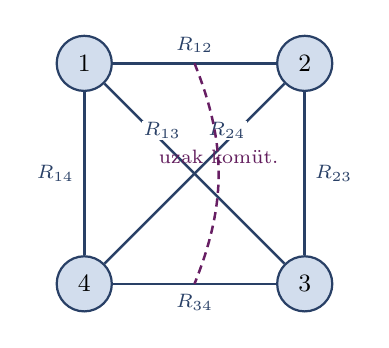
\begin{tikzpicture}[x=1.4cm,y=1.4cm]
  \node[knode] (n1) at (0,2) {1};
  \node[knode] (n2) at (2,2) {2};
  \node[knode] (n3) at (2,0) {3};
  \node[knode] (n4) at (0,0) {4};
  % 6 kenar = 6 R_{ij}
  \draw[kedge] (n1)--(n2) node[midway,above,font=\scriptsize]{$R_{12}$};
  \draw[kedge] (n2)--(n3) node[midway,right,font=\scriptsize]{$R_{23}$};
  \draw[kedge] (n3)--(n4) node[midway,below,font=\scriptsize]{$R_{34}$};
  \draw[kedge] (n1)--(n4) node[midway,left,font=\scriptsize]{$R_{14}$};
  \draw[kedge] (n1)--(n3) node[pos=0.32,above,font=\scriptsize,fill=white,inner sep=0.5pt]{$R_{13}$};
  \draw[kedge] (n2)--(n4) node[pos=0.32,above,font=\scriptsize,fill=white,inner sep=0.5pt]{$R_{24}$};
  % uzak komutativite vurgusu (12)-(34)
  \draw[faredge] ($(n1)!0.5!(n2)$) to[bend left=22] node[above,font=\scriptsize,oddsign!70!black]{uzak komüt.} ($(n3)!0.5!(n4)$);
\end{tikzpicture}
\caption{$V^{\otimes 4}$ yerleşimlerinin $K_4$ grafiği: altı kenar altı $R_{ij}$,
dört üçgen ($\{1,2,3\},\{1,2,4\},\{1,3,4\},\{2,3,4\}$) dört lokal Yang--Baxter
kontrolü, ayrık kenar çifti $(12)\,$--$\,(34)$ ise uzak komütativitedir.}
\label{fig:k4}
\end{figure}

Dört üçlü altblok kontrolü tek bir fonksiyonda toplanır; bu fonksiyon
\texttt{tests/test\_supergroup\_gl21.py} içindeki dört faktörlü yerleşim
testleriyle birlikte çalıştırılır:

\begin{pythoncode}{$V^{\otimes 4}$ içindeki dört üçlü için lokal YBE kontrolü}
def local_ybe_on_four_tensor_GLq21(q_sym=q):
    Rij = all_Rij_GLq21(4, q_sym)          # six 81x81 placements
    result = {}
    for a, b, c in combinations(range(4), 3):   # (0,1,2),(0,1,3),(0,2,3),(1,2,3)
        Rab, Rac, Rbc = Rij[(a, b)], Rij[(a, c)], Rij[(b, c)]
        residual = Rab*Rac*Rbc - Rbc*Rac*Rab
        result[(a, b, c)] = _is_zero_matrix_symbolic(residual)
    return result
\end{pythoncode}

\begin{table}[h]
\centering
\small
\caption{$V^{\otimes 4}$ üzerindeki $81\times 81$ yerleşimler ve otomatik
kontroller.}
\label{tab:vtensor4}
\begin{tabularx}{\textwidth}{@{}l l X@{}}
\toprule
Kontrol & İlgili operatörler & Anlamı \\
\midrule
Yerleşimler & $R_{12},R_{13},R_{14},R_{23},R_{24},R_{34}$ & $K_4$'ün altı kenarı \\
\addlinespace[1pt]
Lokal YBE $\times 4$ & üçlüler $(a,b,c)$ & $R_{ab}R_{ac}R_{bc}=R_{bc}R_{ac}R_{ab}$ \\
\addlinespace[1pt]
Uzak komütativite & $R_{12},R_{34}$ & ayrık kenarlar komüte eder \\
\bottomrule
\end{tabularx}
\end{table}

\subsection{Metodolojik Katkı}

Bu bölümün kazanımı yöntemseldir. Literatürde verilen $GL_q(2|1)$
$R$-matrisinin graded Yang--Baxter denklemine ilişkin uzun matris hesabı,
burada açık kaynaklı, test edilebilir ve yeniden üretilebilir bir sembolik
doğrulama prosedürüne dönüştürülmüştür. Sonuç, soyut Hopf süpercebir
aksiyomlarının tam sınıflandırması değil; açık baz, açık parite ve açık
süper permütasyon seçimi altında yürütülen temsil düzeyinde bir kalıntı
kontrolüdür.

\section{Klasik, Kuantum ve Birim Kök Limitleri}\label{sec:limits}

Son hesaplamalı katkı, aynı $V_n$ temsilini üç farklı asimptotik rejimde yan
yana koyarak ``kuantize etmenin'' somut anlamını göstermektir. Bu bölümdeki
hesaplar genel bir birim-kök temsil teorisi kurmaz; yalnızca klasik limit,
formel genel $q$ ve seçilmiş bir birim-kök özelleştirmesinde açık matrislerin
nasıl değiştiğini izler.

\subsection{(L1) Klasik Limit $q \to 1$}

Cartan elemanını şu limitle geri kazanırız:
\[
  h := \lim_{q \to 1} \frac{K - 1}{q - 1}.
\]
Köşegen olduğu için $h$'nin $k$. girişi
$\lim_{q \to 1} (q^{n-2k} - 1)/(q - 1) = n - 2k$, yani klasik
$\sl_2$ ağırlığıdır.

\begin{proposition}[Seçilen temsillerde sayısal doğrulama]\label{thm:classical}
$V_n$ için, $h = \lim_{q\to 1} (K-1)/(q-1)$ ile tanımlanan operatörün
köşegen girişleri $\{n, n-2, n-4, \dots, -n\}$'dir; ve aynı limit
$\lim_{q\to 1} [E,F] = h$ olur.
\end{proposition}

Doğrulama, $V_1, V_2, V_3, V_4$ için \path{tests/test_limits.py}
içindeki \path{test_classical_commutator_equals_h} testi ile
yapılmıştır.

\subsection{(L2) Genel $q$}

Çalışmanın büyük kısmının yürüdüğü asıl kuantum rejim budur. $K$-özdeğerleri
$\{q^n, q^{n-2}, \dots, q^{-n}\}$, $E$-katsayıları ise $\qint{k}\qint{n-k+1}$
biçimindedir. Burada $q$ birim kökü olmadığından temsil teorisi klasik durumun
``düzgün'' bir deformasyonudur: $V_n$ indirgenemez kalır, dört bağıntı ve dokuz
Hopf aksiyomu sembolik $q$ üzerinde sağlanır.

\subsection{(L3) Birim Kök $q^N = 1$}

$q$ bir $N$. primitif birim kökü $\zeta = e^{2\pi i/N}$ ile değerlendirildiğinde
$\qint{N}=0$ olur ve genel-$q$ resmi köklü biçimde değişir. $E^N$, $F^N$ ve
$K^{2N}$ merkezîleşir; bazı $\qint{k}\qint{n-k+1}$ katsayıları sıfırlandığından
daha önce indirgenemez olan kimi $V_n$ temsilleri parçalanabilir hâle gelir.
Yani deformasyonun ``zararsız'' göründüğü genel rejimden, temsil teorisinin
yeniden kurulmasını gerektiren bir rejime geçilir.

\begin{example}[Sayısal gözlem]
$N = 4$ alalım, yani $q = i$. $V_2$ üzerinde $E$-matris katsayıları
$\qint{1}\qint{2}$ ve $\qint{2}\qint{1}$ formundadır. Burada
\[
  \qint{2} = q + q^{-1} = i + i^{-1} = 0
\]
olduğundan, hesaplama $E = 0_3$ verir:
\[
  E\big|_{q=i} = \begin{pmatrix} 0 & 0 & 0 \\ 0 & 0 & 0 \\ 0 & 0 & 0 \end{pmatrix}.
\]
Yani $V_2$, $q = i$'de yapısal olarak \emph{çöker} ve genel $q$
durumundakinden farklı, indirgenebilir bir $\Uq|_{q=i}$-modül hâline
gelir. Bu olgu \path{tests/test_limits.py::test_root_of_unity_V2_at_q4_singular}
ile sayısal olarak doğrulanmıştır.
\end{example}

Bunun teorik arka planı, Lusztig'in birim-kök ve küçük kuantum grup
$u_q(\sl_2)$ kuramıyla ilişkilidir \cite{Lusztig}. Bu makaledeki kod ise bu
kuramı inşa etmez; yalnızca seçilen temsilde katsayıların sıfırlanmasıyla ortaya
çıkan temsil düzeyindeki tekil davranışı kaydeder.

\subsection{(L4) Kristal Limit $q \to 0$}

Üçüncü teorik bölümde tartışılan kristal taban, aslında $q\to 0$ limitine
karşılık gelir \cite{Kashiwara,HK}. Bu rejimde tekil matris katsayıları ıraksasa da $V_n$'in
kombinatoryal gölgesi --- kristal $B(n)$ ---
\[
  b_0 \xrightarrow{\tilde f} b_1 \xrightarrow{\tilde f} \dots
   \xrightarrow{\tilde f} b_n
\]
yolu olarak ayakta kalır; $\tilde f$, $F$-eyleminin tek bir oka indirgenmiş
hâli, $\tilde e$ ise tersidir. Pakette bu yapı \texttt{quantum\_group/crystal.py}
modülünde bir grafik nesnesi olarak kurulur ve görselleştirilir.

\subsection{Üç Limitin Karşılaştırması ($V_2$ örneği)}

\begin{table}[h]
\centering
\small
\caption{$V_2$ temsilinin üç limit rejimindeki karşılaştırması.}
\label{tab:limits}
\begin{tabularx}{\textwidth}{@{}lXXX@{}}
\toprule
& Klasik ($q \to 1$) & Genel $q$ & Birim kök ($q^4 = 1$) \\
\midrule
$K$-özdeğerleri & 1, 1, 1 & $q^2, 1, q^{-2}$ & $-1, 1, -1$ \\
$h$-özdeğerleri & 2, 0, $-2$ & --- & --- \\
$E$-girdileri & 2, 2 & $\qint{1}\qint{2}, \qint{2}\qint{1}$ & 0, 0 \\
İndirgenemez mi? & Evet & Evet & \textbf{Hayır} \\
Boyut & 3 & 3 & 3 \\
\bottomrule
\end{tabularx}
\end{table}

Bu karşılaştırma, tek bir temsil üzerinde $q$ parametresinin üç farklı rolünü
ayırır: klasik limitte ağırlıklar geri kazanılır, genel $q$'da katsayılar
$q$-tamsayılarla deforme olur, birim kökte ise bazı katsayılar sıfırlanarak
temsil düzeyinde yeni tekillikler doğar.

\section{Sonuçlar ve Gelecek Çalışma}

Bu çalışmada $\Uq$ kuantum grubu ile $GL_q(2|1)$ kuantum süpergrubu, aynı
sembolik sıfır-kalıntı doğrulama çekirdeği üzerinden ele alındı. Elde edilen
hesaplamalı sonuçlar şöyle özetlenebilir:

\begin{itemize}[leftmargin=*]
  \item \textbf{$\Uq$ temsilleri}: Sonlu boyutlu $V_n$ temsilleri açık
        matrislerle uygulandı; $E,F,K,K^{-1}$ operatörleri ve ağırlık verileri
        tek bir temsil nesnesinde toplandı.
  \item \textbf{Bağıntılar ve Hopf yapısı}: Dört (R1)--(R4) bağıntısı ve Hopf
        yapısı, seçilen sonlu boyutlu temsiller üzerinde sembolik
        sıfır-kalıntı testleriyle doğrulandı.
  \item \textbf{Tensör teorisi}: $V_m \otimes V_n$ üzerinde eş-çarpımdan gelen
        eylem kuruldu; Clebsch--Gordan ayrışımının en yüksek ağırlık vektörleri
        $q$-deforme katsayılarıyla elde edildi.
  \item \textbf{$R$-matrisi ve örgü bağıntıları}: $V_1 \otimes V_1$ üzerinde
        $R$-matrisi, kuantum Yang--Baxter denklemi, örgü bağıntısı ve Hecke
        bağıntısı hesaplamalı olarak kontrol edildi.
  \item \textbf{Graded durum}: Salih Çelik ve Sultan A.\ Çelik'in
        $GL_q(2|1)$ $R$-matrisi için graded Yang--Baxter denklemi, parite
        uyumlu süper permütasyonla kurulan $R_{13}$ yerleşimi kullanılarak
        $27\times 27$ kalıntı matrisinin tüm girdileri düzeyinde sıfıra
        sadeleştiği görüldü.
  \item \textbf{Yeniden üretilebilirlik}: Raporlanan kontroller
        \texttt{pytest} testlerine bağlandı; şekiller ve PDF çıktısı depo
        içindeki betikler ve \texttt{Makefile} hedefleriyle yeniden üretilebilir
        hâle getirildi.
\end{itemize}

$\Uq$ tarafındaki kazanç, klasik temsil teorisini $R$-matrisi/örgü altyapısıyla
tek bir test edilebilir pakette buluşturmaktır. $GL_q(2|1)$ tarafında ise asıl
katkı yöntemseldir: literatürdeki uzun graded Yang--Baxter hesabı, açık baz,
açık parite ve açık süper permütasyon üzerinden yeniden üretilebilir bir sembolik
prosedüre dönüşür. Sonuçların tamamı --- \texttt{tests/} birim testleri,
\texttt{requirements.txt} bağımlılıkları, LaTeX kaynağı ve üretilen PDF --- depo
klonlanarak yeniden elde edilebilir.

Bu yaklaşım, yüksek boyutlu Yang--Baxter tipi hesapların elle yürütülen
cebirsel manipülasyonlardan, test edilebilir ve yeniden üretilebilir sembolik
doğrulama prosedürlerine taşınabileceğine dair somut bir örnek verir.

\paragraph{Sınırlılıklar.}
Bu çalışma temsil düzeyinde sembolik doğrulamalar yapar; soyut evrensel cebir
düzeyinde tam bir ispat asistanı değildir. Sembolik sadeleştirme, özellikle
$V^{\otimes n}$ boyutu büyüdükçe hızla maliyetli hâle gelir. Jones polinomu
hesaplaması ve Markov izi uygulanmamıştır; yalnızca örgü ve Hecke bağıntıları
kontrol edilmiştir. Birim-kök davranışı seçilmiş örnekler üzerinden
gösterilmiştir; küçük kuantum grup kuramı tam olarak uygulanmamıştır. Kristal
tarafında paket $B(n)$ kombinatoryal grafiğini kurar, Kashiwara global bazını
inşa etmez. $GL_q(2|1)$ doğrulaması ise kullanılan baz sıralamasına ve
$p(e_1)=p(e_2)=0$, $p(e_3)=1$ parite konvansiyonuna bağlıdır.

\paragraph{İleri çalışma yönleri.}
\begin{enumerate}[leftmargin=*]
  \item \emph{Jones polinomu hesaplaması}: bu çalışmadaki örgü temsilini Markov
        izi ile birleştirerek küçük düğümlerin (trefoil, sekiz-düğüm) Jones
        polinomunu hesaplama.
  \item \emph{Yüksek rank}: $U_q(\sl_n)$ ve genel Cartan tipi için aynı
        altyapının genelleştirilmesi.
  \item \emph{Küçük kuantum grup}: $u_q(\sl_2)$'nin birim kökünde tam
        temsil teorisinin ve blok yapısının inşası.
  \item \emph{Crystal tensör çarpımı}: $B(m) \otimes B(n)$ kristal
        kuralının uygulanması ve klasik Clebsch--Gordan ile karşılaştırılması.
  \item \emph{Gauss ayrışımı ve Hopf süpercebir}: $GL_q(2|1)$ için
        makaledeki Gauss ayrışımı, üst/alt üçgensel alt süpergruplar, RTT
        bağıntıları ve Hopf süpercebir eşlemelerinin kodla doğrulanması.
\end{enumerate}

\appendix
\section{Kod ve Tekrar Üretilebilirlik}

Tüm kaynak kod GitHub deposunda açık olarak bulunmaktadır:
\url{https://github.com/TerekliTahaBerk/quantum-groups}.

\paragraph{Kurulum.} Python 3.10+ önerilir; paket SymPy, NetworkX, Matplotlib,
pytest ve Jupyter bağımlılıklarını \texttt{requirements.txt} üzerinden kurar.
\begin{bashcode}
python3 -m venv .venv
source .venv/bin/activate
python3 -m pip install -r requirements.txt
\end{bashcode}

\paragraph{Testler.} Tüm doğrulamalar \texttt{pytest} ile çalıştırılır.
\begin{bashcode}
python3 -m pytest tests/ -q
\end{bashcode}

\paragraph{Demo.} Uçtan uca gösterim betiği çalıştırılır.
\begin{bashcode}
python3 main.py
\end{bashcode}

\paragraph{Şekiller.} Makaledeki PDF şekilleri aynı betikle yeniden üretilebilir.
\begin{bashcode}
python3 thesis/figures/generate_figures.py
\end{bashcode}

\paragraph{PDF derleme.} Tectonic (XeTeX tabanlı) Türkçe/Unicode metni doğrudan
derler. Bu revize sürüm için kullanılan komut şöyledir:
\begin{bashcode}
tectonic thesis/thesis_revised.tex
\end{bashcode}

\paragraph{Kolaylık hedefleri.} Aynı işlemler \texttt{make} ile de yapılabilir.
\begin{bashcode}
make test    # pytest ile tum testler
make pdf     # tectonic ile PDF + yayin adiyla kopya
make demo    # uctan uca demo
\end{bashcode}

\paragraph{Temel doğrulama çağrıları.} Üç ana eşitlik, paket içe aktarıldıktan
sonra üç satırda denetlenebilir.
\begin{pythoncode}{Temel doğrulama çağrıları}
assert qybe_holds(R_matrix_V1())
assert graded_yang_baxter_holds_GLq21()
assert all(local_ybe_on_four_tensor_GLq21().values())
\end{pythoncode}

\paragraph{Ad uyumluluğu.} Makale taslaklarında kullanılan
\path{build_representation_core} ve \path{verify_relations_core}
adları, depoda geriye uyumlu public sarmalayıcılar olarak korunur; kararlı API
adları sırasıyla \path{build_representation} ve
\path{verify_on_representation} fonksiyonlarıdır.

\section{Test Eşlemesi}

Her doğrulama ekseni, ilgili kod modülü ve birim test dosyasıyla
Tablo~\ref{tab:tests}'te eşlenmiştir.

\begin{table}[H]
\centering
\footnotesize
\caption{Doğrulama eksenleri, kod modülleri ve test dosyaları.}
\label{tab:tests}
\begin{tabularx}{\textwidth}{@{}>{\raggedright\arraybackslash}p{0.24\textwidth}X>{\raggedright\arraybackslash}p{0.30\textwidth}@{}}
\toprule
Doğrulama & Kod Modülü & Test Dosyası \\
\midrule
$U_q(\sl_2)$ bağıntıları & \texttt{relations.py} & \texttt{test\_relations.py} \\
Hopf aksiyomları & \texttt{hopf.py} & \texttt{test\_hopf.py} \\
Temsiller ve kristaller & \texttt{representations.py}, \texttt{crystal.py} & \texttt{test\_representations.py} \\
Clebsch--Gordan & \texttt{tensor.py} & \texttt{test\_tensor.py} \\
R-matrisi/QYBE & \texttt{r\_matrix.py} & \texttt{test\_r\_matrix.py} \\
$GL_q(2|1)$ graded YBE & \texttt{supergroup\_gl21.py} & \texttt{test\_supergroup\_gl21.py} \\
Limit analizleri & \texttt{limits.py} & \texttt{test\_limits.py} \\
\bottomrule
\end{tabularx}
\end{table}

\FloatBarrier
\begin{thebibliography}{9}
\bibitem{Drinfeld}
V.~G.~Drinfeld, \emph{Quantum Groups}, Proceedings of the International Congress of Mathematicians, Berkeley, 1986.

\bibitem{Jimbo}
M.~Jimbo, \emph{A $q$-difference analogue of $U(\gfrak)$ and the Yang--Baxter equation}, Lett.\ Math.\ Phys.\ \textbf{10} (1985), 63--69.

\bibitem{Kassel}
C.~Kassel, \emph{Quantum Groups}, Graduate Texts in Mathematics 155, Springer, 1995.

\bibitem{ChariPressley}
V.~Chari, A.~Pressley, \emph{A Guide to Quantum Groups}, Cambridge University Press, 1994.

\bibitem{KS}
A.~Klimyk, K.~Schm{\"u}dgen, \emph{Quantum Groups and Their Representations}, Springer, 1997.

\bibitem{Lusztig}
G.~Lusztig, \emph{Introduction to Quantum Groups}, Birkh{\"a}user, 1993.

\bibitem{Kashiwara}
M.~Kashiwara, \emph{On crystal bases of the $q$-analogue of universal enveloping algebras}, Duke Math.\ J.\ \textbf{63} (1991), 465--516.

\bibitem{HK}
J.~Hong, S.-J.~Kang, \emph{Introduction to Quantum Groups and Crystal Bases}, AMS, 2002.

\bibitem{Jones}
V.~F.~R.~Jones, \emph{A polynomial invariant for knots via von Neumann algebras}, Bull.\ Amer.\ Math.\ Soc.\ \textbf{12} (1985), 103--111.

\bibitem{CelikGL21}
S.~Celik, S.~A.~Celik, \emph{A new quantum supergroup and its Gauss decomposition}, Rep.\ Math.\ Phys.\ \textbf{88} (2021), no.~2, 259--272.

\bibitem{SymPy}
A.~Meurer et~al., \emph{SymPy: symbolic computing in Python}, PeerJ Computer Science \textbf{3} (2017), e103.

\bibitem{pytest}
H.~Krekel et~al., \emph{pytest documentation}, \url{https://docs.pytest.org/}.
\end{thebibliography}

\end{document}
